\documentclass{KU2}
\usepackage{geometry}
\geometry{
 a4paper,
 textwidth=14.2cm,
 top=6.5cm,
 left=4.5cm,
}
\usepackage{hyperref}
\usepackage{setspace}
\usepackage[dvipdfm]{graphicx}
\usepackage{caption}
\usepackage{xeCJK}
\setCJKmainfont{Hiragino Kaku Gothic Pro}

\usepackage{enumitem,amssymb}
\newlist{todolist}{itemize}{2}
\setlist[todolist]{label=$\square$}
\usepackage{pifont}
\newcommand{\cmark}{\ding{51}}%
\newcommand{\xmark}{\ding{55}}%
\newcommand{\done}{\rlap{$\square$}{\raisebox{2pt}{\large\hspace{1pt}\cmark}}}%

\usepackage[ruled]{algorithm2e}
\SetKw{KwInit}{Init}

\begin{document}

\title{Methods of Deciding Annotation Order\\for Efficient Target-Data Extraction\\in Supervised Machine Learning\\}
\author{Ruide Li}
\supervisor{Keishi Tajima}
\setdegree{Master}
\maketitle

\large
\onehalfspacing

\begin{abstract}
In this research, I propose several methods of deciding annotation order when a dataset is given to extract data of a target class using supervised machine learning.

As the boosting development of supervised machine learning, models are becoming more and more hungry for labeled training data. Since human annotation may cost a huge amount of time and money, in order to train a classifier with acceptable performance using as few human annotations as possible, it is effective to give priority to each sample and make samples with higher priority to be labeled sooner. To handle this kind of problem, it is possible to make use of active learning algorithms. However, most existing research is designed for general applications on arbitrary tasks, while in actual application, it is possible to make use of the data specific properties since the purpose of the task and the data format are given on most occasions. Furthermore, besides typical active learning, this research also aims to find data of a specific target with as few annotation work as possible since there is a need for speedy extracting data of a certain target class on some occasions. In this research, I mainly focus on document classification tasks such as spam/ham SMS message and positive/negative movie review.

There are three main purposes in my research. First, I introduce text-based properties to improve active learning algorithms. I hypothesize that if the model can learn documents with more informative words at first, it can contribute more to the goals. I propose several approaches to measure the informative level of a document, making use of bag-of-words feature count, tf-idf score and norm of Doc2Vec vector. I use existing algorithms such as uncertainty sampling to find several candidates, and then take more informative ones for human annotation. In experiments, proposed methods were evaluated to give to 5--10\% better f1-score than naive methods.

Second, I propose a method for collecting more target data with fewer annotation work. Till there is enough data with label, the system iteratively finds target likely samples as candidates, from which the most informative one will be taken for human annotation. At the meantime, it also keeps updating the model using the current labeled data to revise the data priority. And at the point that the system judges the classification model obtains a sufficiently high performance, the system switches the worker from human annotation to the classifier so that the human annotators contribute to the next new tasks. Experimental results have shown up to 5\% faster speed on different datasets.

Third, through the research of the first and the second purposes, there comes a dilemma between querying a label for a data which is likely to be a target data and querying for a data which is likely to improve the classifier. In this part, I will indicate the dilemma by showing experimental results. Furthermore, in real applications, operators may need information about the performance of obtained model in order to decide when to switch from human annotation to model prediction. So I also propose a framework which can provide curves of several metrics, trying to give a feedback to the operators. Also, I will discuss the estimation about the current model using regular phenomena I have found from the experiments.

\pagebreak

\begin{center}
\begin{huge}
  \textbf{教師あり機械学習における効率的な目標\\データ抽出のためのタグ付け順序決定手法\\}
\end{huge}
\end{center}

\begin{flushright}
\textbf{李 瑞徳}
\end{flushright}

\begin{flushleft}
\textbf{和文梗概}
\end{flushleft}

あるラベルなしデータ集合が与えられたときに、特定のクラスのデータを早く収集したい場合(以降、これを「ターゲットクラス」と呼ぶ)、無作為な順番でアノテータにタグ付けさせるのではなく、何らかの「ターゲットクラスらしさ」の情報を使ったり、すでにタグ付けされたデータで学習した分類器を使って、タグ付けさせる順番を決めることが有効であると考えた。このようなアイディアの元、本研究では、効率的にターゲットクラスのデータを収集することを目的として、タグ付けの順序を決定する手法を提案する。

教師あり機械学習の急速な発展に伴い、ラベル付きトレーニングデータの需要が高まっている。人間によるタグ付けは、タスクやそのデータサイズによっては膨大な時間と費用がかかるので、より少ないデータへのタグ付けでより高い性能を持つ分類器を学習するために、サンプルに優先順位を付け、優先度の高いサンプルを先にラベリングさせるのがより効率的になる。このような問題を解決するのに、能動学習手法を利用することが可能である。しかし、既存の能動学習のほとんどは任意のタスクで動作するよう汎用的に設計されているが、実際の応用では、タスクの目的やデータ形式はあらかじめ決められている場合が多いので、そのデータ特有の性質を利用することが可能である。このようなデータ特有の情報は、そのメディアの種類に応じて様々考えられるが、本研究はSMSメッセージのスパム分類と映画レビューのセンチメント分類のような文書分類タスクに注目する。

本研究で具体的には以下の三つを目的とする。まず、一つ目の目的は、テキストデータの属性を用いて能動学習手法を改善する。モデルは情報量の高い単語を含む文書をより先に学習できるなら、より早く高い性能に達成できるという仮説を立てる。したがって、tf-idfスコアや単語の埋め込みなど、テキスト特有の特性を利用し、文書の情報量を推定する手法を提案する。Uncertainty Samplingなどの既存アルゴリズムで候補者を絞り込み、その中から情報量の高い文書を選んで先にタグ付けをする。実験では、提案の結合手法が単純手法より5—10\%高い性能を出せることが検証できた。

二つ目の目的は、タグ付けさせるデータの順位を決定することで、少ないデータでより高い性能のモデルを獲得することである。モデルの性能を向上させるのに効果があるのは、より情報量の高い単語を含む文書であると考えた。文書の情報量を推定する手法を提案し、既存のアルゴリズムと組み合わせて効果を評価する。実験結果は、これらの組み合わせ手法はベースラインより高い性能を与えることを示した。提案手法では、学習モデルの精度が低いうちは、システムが学習モデルを使って算出した優先順位に従ってアノテータにタグ付けさせ、そのたびにそれまでに得られたタグ付けデータを使用してモデルを更新する。そして、学習モデルが十分に高い性能を獲得したと判断した時点で、システムは人間のタグ付けから学習モデルによる自動タグ付けに切り替える。これにより、人間は別のタスクに貢献することができるだろう。このようにして、タグ付けコストを削減する一方で、できるだけ多くのターゲットデータを取得する。複数データセットで実験した結果、提案の結合手法は単純手法より、最大5\%高い性能を出せることが分かった。

三つ目の目的は、データの数があまり多くない場合、ターゲットデータを優先してタグ付けすると、タグ付けデータにおけるターゲットデータの比率は当然上がるが、これからタグ付けしようとするデータにおけるターゲットデータの比率は下がることになるため、データ間にミスマッチが起きて学習データの性能が低下するというジレンマを分析し、その解決手法を提案することである。実験によってこのジレンマにおけるモデルのふるまいを示す。更に、実際の応用で、オペレータはリアルタイムに当時点のモデルに関する評価指標が分かる必要がある。なぜなら、どのようなタイミングでモデルの予測に切り替えることが判断しないといけないからである。なので、各指標の曲線を提供し、オペレータにフィードバックできるようなフレームワークも提案する。また、実験から得られた規則的な現象を用いて、二つ目の目的で提案したアルゴリズムを改良する手法についても論じる。
\end{abstract}

\tableofcontents

\chapter{Introduction}
As the boosting development of supervised machine learning, models are becoming more and more hungry for labeled training data. If people want to extract data from a certain target class when a pool of unlabeled data is given, usually human annotation is required at first to train a classifier. Data labeling tasks can be finished by experts (technical problems such as medical or geological image analysis), trained employees (less technical, but needs formal training, for some financial problems), or normal web users (crowdsourcing, relatively simple problems, but need a lot of effort to deal with spammers). All of these labeling methods may cost a huge amount of money and time. So it will be helpful if there are some methods that can reduce this labeling cost, with the assurance of same-level performance of the model. I discuss the problem of extracting target data efficiently, for example, imagine a task of Twitter mining for rescue information in disasters. So from this aspect, I focus on text data such as documents and messages since text is frequently used for active learning tasks.

To handle the problem of annotation cost reduction, many active learning algorithms have been developed, so that models can achieve equal or better accuracy using much less labeled training data \cite{survey}. In the pool-based active learning problem \cite{settles}, it is usually to have a pool of unlabeled data, and the pick up a sample from the pool for human annotation, referring to a decision function which gives the priority of every sample. Existing researches mainly focus on arbitrary data to give generalized approaches on arbitrary tasks, while in actual application, the purpose of task and data format are given on most occasions. Hence, it is possible to make use of the properties of data. Different kinds of media have different features, if I can make use of these features, can I improve the model better than generalized approaches? In this research, I proposed some approaches specially designed for text data, using text-base properties. The hypothesis is that, for a document classification problem, the model may learn faster if I feed more informative data to the model at the early phase. I discuss several ways of measuring how informative a document could be, and give higher priority of annotation to informative data.

Furthermore, besides the performance of the model, there is a need for speedy extracting data of a certain target class on some occasions. However, in typical active learning problem, the speed of finding target data is not taken into consideration. So in this research, I do not only focus on the aspect of active learning, but also try to find data from a specific target class as soon as possible. When there is enough data with label, the system lets annotators give labels according the priority order and also keep updating the model using the current labeled data to revise the data priority. And at the point that the system judges the classification model obtains a sufficiently high accuracy, the system switches the worker from the human annotations to the classifier so that the human annotators contribute to the next new tasks. In this way, in the meantime of reducing human annotation cost, it is able to get as many target data as possible.

\section{Purposes of This Research}
Usually, if we try to efficiently extract data from a certain target class from a pool of unlabeled data using as few human annotation as possible, there may be several approaches we can think about. I mainly discuss three purposes in my research, and I will discuss these three purposes separately in the following subsections. Notice that in active learning, people do not consider the quality of human annotation. In my research, I use similar context, assuming human annotation as ground truth.

\subsection{Improving Performance of Obtained Model}
First of all, it is possible to use active learning algorithms to improve the model with less human annotation. For instance, uncertainty sampling \cite{uncertainty}, in which samples will be annotated earlier if the model gives it a confidence close to random guess, is a well-known approach in active learning problem. The intuition is that, if the model is not sure about a certain sample, the model may learn better if people feed these ``difficult'' samples to the model earlier. In this way, people may quickly get a model with acceptable performance, and use this model to predict target data from unlabeled data pool. So from the aspect of active learning, I try to make use of these text-base properties to improve the model, focusing on improving the performance of obtained model.

\subsection{Finding Data from Target Class Faster}
In the pool-based active learning problem \cite{survey}, it is usually to have a pool of unlabeled data, and the pick up a sample from the pool for human annotation, referring to a function which gives the priority of every sample, while in this purpose, I discuss a problem of collecting target data from a fixed pool of unlabeled dataset as fast as possible by using machine learning but not focusing on the performance of the model. I query human annotators for the label of a chosen candidate data one by one to find target data, and I also use the obtained labels to train a classifier, which is used for choosing the next candidate. This problem is different from the ordinary active learning problem in several ways. First, my goal is to collect target data as fast as possible (i.e., with as few queries for non-target data), while in the active learning I want to minimize the total number of both target and non-target queries. Second, the active learning problem focuses on the performance of the obtained classifier, while it is not important in my problem as long as I can collect target data fast. I call this problem target-retrieval-learning problem.

Uncertainty sampling \cite{uncertainty}, in which samples with lower confidence will be annotated earlier, is a well-known approach in the ordinary active learning problem, existing research has shown that the opposite approach, which gives higher priority to samples with higher confidence, is a better strategy \cite{enumerate}.

\subsection{Tackling the Performance-Target Dilemma}
Furthermore, due to expensive human annotation cost, I want to train a supervised machine learning model on the labeled data, and let the model to predict the class of the remaining unlabeled data. The model should give a feedback of how the model will perform on the remaining unlabeled data, and provide a ranking of likelihood of target data.

However, One issue in the target-retrieval-learning problem is the difficulty of estimating the performance of the obtained classifier on the remaining data. It is difficult because the labeled data in my problem is biased towards target data, while the remaining data is biased towards non-target data. This becomes a problem if I want to know on what point I can trust the classifier and switch from human annotation to the obtained classifier.

As a result, there is a dilemma between querying a label for a data which is likely to be a target data and querying for a data which is likely to improve the classifier. Moreover, the classification boundary of the classifier is not important in my problem as long as the best candidate chosen by the classifier in each step is always a target data.

To solve the dilemma, I try to estimate the performance of obtained model on unlabeled data, or provide a ranking of target likelihood of unlabeled data.

\section{Application Scenario}
For a scenario of potential application, I imagine Twitter mining for rescue information in disasters. People may post tweets for asking rescue, or providing information about the disaster area. Suppose I want to train a model to classify this relevance problem, it is nearly impossible to label all tweets during that urgent period of time. During the early phase, I may use target-retrieval-learning algorithm to retrieve relative tweets as many as possible for annotation, and use these labeled data as training set to train a classifier. At certain point, I may switch to the classifier to finish the job without human annotation, only if I can estimate the performance of the classifier on the whole population.

\subsection{Improving Performance of Obtained Model}
The simplest way to deal with this is to train a machine learning model. So in order to training the model faster and cheaper, active learning algorithms can be used during annotation process. The purpose of human annotation is just to give data labels, so that the dataset can be used to train a supervised machine learning model.

\subsection{Finding Data from Target Class Faster}
However, in this case, target data is much more valuable than non-target data, since rescue action should be taken rapidly if a rescue tweet is found. So from this aspect, the model should try to find target data as soon as possible, and I not only want the human annotator just to give a label, but also give a check whether the model is giving right target data or not. In this way, I am able to get target data with much less non-target annotation.

At the meantime, I also have labeled data which can be used to train a classifier. As labeled data accumulates, I may want to switch to the classifier to finish the job when the model is well learned.

\subsection{Tackling the Performance-Target Dilemma}
So here comes a problem: how can I estimate whether the model is well learned? There should be some feedback metrics during the annotation process, so that I can observe these metrics and give an estimation. When the model gives acceptable performance, there is no need to do human annotation any more. The model should provide a ranking of the likelihood of target class, and rescue action would be done in the order of target likelihood ranking. In this way, I am able to both find more target data and reduce the cost of human annotation.

\section{Structure of This Thesis}
In the next chapter, it will show some related literatures which provides approaches about active learning problem, reducing annotation cost with specified purpose and improving training speed. And then, I explain a framework I have built for annotation process simulation, which is specially designed for this research. As for my proposed approaches, I discuss separately in three section for the three purposes mentioned above. In the experiments chapter, I show the results of proposed approaches using the simulation framework on three datasets. Furthermore, in order to analyze the effects of unbalance factor, I did my experiments several times with manually changing the proportion of target data. Finally, I conclude what I can know from the experiment result and discuss some further issues about this research.

\chapter{Related Work}
In this chapter, I first introduce several basic concepts in active learning, and then I discuss some well known approaches both in ordinary active learning problem and variant problem similar to active learning. Finally, I also mentioned an approach which focuses on improving training speed instead of reducing annotation cost.

\section{Active Learning}
As I all know, for training a supervised machine learning model human annotation may cost a huge amount of money and time. Moreover, because of the boost of algorithms using neural network, models are even more hungry for labeled data. As one of the solution to this problem, many active learning algorithms have been developed, so that models can achieve equal or better accuracy using much less labeled training data. To do literature search about existing researches, I go through a literature survey about active learning algorithms \cite{settles}. In this literature survey, the author summarized three typical categories of active learning algorithm: pool-based (the pick up a sample from the pool of unlabeled data by means of a querying function), stream-based (the tells whether to do annotation in a stream of unlabeled data) and membership queries (the generates data from the feature space of unlabeled data).

In active learning, I usually call a human annotator as an ``oracle'' \cite{settles}, assuming that the oracle always gives the ground truth label. There are three major approaches in active learning: pool-based, stream-based and membership queries. In pool-based active learning, the active is provided with a pool of independent and identically distributed unlabeled instances. The active at each step chooses an unlabeled instance to request the label from the oracle by means of a querying function. This is also called as selective sampling. Furthermore, stream-based approaches, can be considered as an online version of pool-based approaches. The active is presented with a stream of unlabeled instances, in which the active gives a yes/no decision whether the coming unlabeled instance should be labeled by the oracle or not. Finally, as for active learning with membership queries, the active asks the oracle to classify instances generated by the learning system. The active imposes values on the attributes for an instance and observes the response. This gives the active the flexibility of framing the data instance that will be the most informative to the active at that moment.

In my research, I find out that the problem is closed to pool-based active learning, especially in the aspect of a fixed pool of unlabeled data which do not change during the annotation phase. As for the differences, typical active learning only focus on the performance of the model, while in my research, I not only try to ensure the performance, but also try to gather target samples at the early phase of annotation as well. Besides, most of active learning approaches focusing on cross-domain, they try to tackle active learning problems with one generally applicable method, so that there will be no need to make such an effort to do manually design and comparison. However, such approaches may focus on the distribution of the data, rather than what the data actually is. These methods rarely make usage of properties of the datasets. But what if I take such properties into consideration? In this research, I proposed some approaches which specially designed for text data, using text-base properties such as bag-of-words, td-idf, Doc2Vec, etc.. From the perspective of typical active learning, I consider the problem quite close to pool-based active learning problem — how to choose next data for oracle labeling from a pool of unlabeled data, since there is no actual need for the online stream. As for membership query, although query synthesis is reasonable for many problems, but labeling such arbitrary instances can be awkward if the oracle is a human annotator. For example, \cite{membership} employed membership query learning with human oracles to train a neural network to classify handwritten characters. They encountered an unexpected problem: many of the query images generated by the active contained no recognizable symbols, only artificial hybrid characters that had no natural semantic meaning. Similarly, I could easily imagine that membership queries for natural language processing tasks might just generate meaningless text that people cannot even read. 

\section{Uncertainty Sampling}
\cite{uncertainty} proposed a heuristic way to decide the order of picking up samples from unlabeled data pool for annotation called ``uncertainty sampling''. Uncertainty sampling is an iterative process of manual labeling of examples, classifier fitting from those examples, and making use of the classifier to select new examples whose class membership is unclear. Their test of this method on a text categorization task showed reductions of up to 500-fold in the number of examples that must be labeled to produce a classifier with a given effectiveness.

Relevance feedback \cite{relevance} does a kind of non-random sampling. In effect, users are asked to label those texts that the current classifier considers most likely to be class members. This approach, which they call relevance sampling, is a reasonable strategy in a text retrieval context, where the user is more interested in seeing relevant texts than in the effectiveness of the final classifier produced. Relevance feedback has also been proposed for finding examples of unusual word senses. However, relevance feedback has many problems as an approach to sampling. It works more poorly as the classifier improves, and is susceptible to selecting redundant examples.

Some other researches like \cite{incremental} give similar strategy if training on misclassified examples, while the difference is that when data is not labeled I must use the classifier itself to guess at which examples are being misclassified. Also, it is worthy to note that in their paper, they mentioned that the initial classifier plays an important role, since without it there may be a long period of random sampling before examples of a low frequency class are stumbled upon.

Since uncertainty sampling is a well-known and robust method, so in my research, I use uncertainty sampling as a baseline of ordinary active learning algorithm.

\section{Balancing Exploration and Exploitation}
Active machine learning algorithms are used when large numbers of unlabeled examples are available and getting labels for them is costly (e.g. requiring consulting a human expert). Many conventional active learning algorithms focus on refining the decision boundary, at the expense of exploring new regions that the current hypothesis misclassifies.

\cite{exploration} proposed a new active learning algorithm that balances such exploration with refining of the decision boundary by dynamically adjusting the probability to explore at each step. Their algorithm addresses active learning problem by randomly choosing between exploration and exploitation at each round, and then receives feedback on how effective the exploration phase was, measured by the change induced in the learned classifier when an exploratory example is labeled and added to the training set. Like a simple reinforcement learning algorithm, their active updates the probability of exploring in subsequent rounds based on the feedback it received.
 
The key idea is that, at each iteration, randomly deciding whether to explore or exploit. If an exploratory step is taken, then their algorithm considers the ``success'' of the exploration to adjust its probability of exploring again. The evaluation of exploration is designed as the cosine similarity between the probabilistic prediction vector on the training set before the exploration step and after. and the probability of exploration is updated by:

 $$p = max(min(p \times exp(\lambda \times d),1 − \epsilon), \epsilon)$$

Here, $p$ is the probability of exploration, $d$ is the scaled cosine similarity, $\lambda$ is the hyperparameter of learning rate, and $\epsilon$ is the upper/lower boundary hyperparameter of the probability.

They first experimented on synthesis 2D/3D checkboard-like data, and then experimented on real world data, and their experimental results demonstrate that improved performance on data sets that require extensive exploration while remaining competitive on data sets that do not, and their algorithm also shows significant tolerance of noise.

However, in some specific fields or dataset, people may be able to tell whether the data requires ``extensive exploration'' or not, such as image segmentation or Statlog (Landsat Satellite) Data Set (from UCI Machine Learning Repository, The database consists of the multi-spectral values of pixels in 3x3 neighborhoods in a satellite image, and the classification associated with the central pixel in each neighborhood. The aim is to predict this classification, given the multi-spectral values.), but if I think of a task of document classification (since I focus on text data in this research), it seems impossible to know in advance whether the dataset requires ``extensive exploration''.

\section{Learning Active Learning from Data}
\cite{lal} proposed a state-of-the-art method in active learning using data-driven approach. Their key idea is to train a regressor that predicts the expected error reduction for a candidate sample in a particular learning state. The motivation is that, existing active learning algorithms suit different situations and many hand-crafted work is needed for a certain application, for instance, different query strategies may work on different datasets, and hyper-parameters should be fine-tuned when the task changes. Furthermore, their experiments indicate that in uncertainty sampling, if the data becomes unbalanced, the ``uncertainty'' probability also changes from 0.5, so it becomes hard to decide how to define the level of ``uncertainty'' when the priori of unlabeled data is not known. In a complex realistic scenario, there are many other factors such as label noise, outliers and shape of distribution that further compound the problem. Although query selection procedures can take into account statistical properties of the datasets and classifier, there is no simple way to foresee the influence of all possible factors. Thus, in their paper, they suggest a meta-learning approach, which they call it ``Learning Active Learning''. It uses properties of classifiers and data to predict the potential error reduction. They tackled the query selection problem by using a regression model; this perspective enables us to construct new active learning strategies in a flexible way. By formulating the query selection procedure as a regression problem they are not restricted to working with existing active learning heuristics; instead, they used strategies based on experience from previous active learning outcomes.

In their experiments they first trained a Random Forest classifier on a synthetic representative dataset to get the loss reduction of each sample as target variables, and used these target variables and pre-designed explanatory variables (mostly meta information of the classifier) to train a Random Forest regressor, and this regressor would become to the querying function to tell annotator which sample to label at each step. Also, they showed that a strategy can be learned either from simple synthetic 2D datasets or from a subset of domain-specific data as representative dataset. Their method yields strategies that work well on real data from a wide range of domains.

However, in my research, I want to investigate whether text-base properties will do any effects in the aspect of active learning, but unfortunately, since in their approach they do not care about the properties of the unlabeled data, only focusing on meta properties of the trained classifier on representative dataset, I cannot use this method as my baseline. In addition, their approach cannot satisfy with my second purpose which tries to find target data faster using as few annotation as possible.
 
\section{Learning to Enumerate}
Besides, there is another variant of typical active learning problem, called ``learning to enumerate'' \cite{enumerate}. The key objective is to find data that satisfies arbitrary but fixed conditions, without using any pre-labeled training data. The key aspect here is to query as few as possible non-target data, while typical active learning techniques try to keep the number of queried labels low they give no regards to the class these instances belong to.

If I had an extensive, labeled dataset to train my model, the best strategy would be to solely rely on its predictions to identify all samples of the target class. However, for when I do not have any labeled data, I am forced to construct my training set from scratch. Sometimes I want to find data satisfying some particular conditions and my goal is to find such data from among the whole dataset. One scenario might be to find high risk patients among a big group of people. Without existing labeled data to train a predictive model, I have to construct a training set, while finding existing high risk patients under the constraint of a limited number of checkups I can perform \cite{predictive}. Yet, only selecting samples which are useful for improving my model does not necessarily comply with my goal to gather all target class samples with as few queries as possible. This is a typical exploitation vs. exploration dilemma that has been studied extensively in reinforcement learning. \cite{enumerate} proposed a simple $\epsilon$-greedy like strategy testing different base s and heuristic functions called learning-to-enumerate. They have experimented on 19 small and mediumsized, public datasets accessible through the UCI Machine Learning Repository. The best results in their experiments were shown by an exploitation only ($\epsilon$ = 0) strategy. Here the exploitation means the model pick up a sample, which has the most highest confidence with the current obtained model.

However, there is a subtle difference in my research from their learning-to-enumerate problem. In their paper, they declare that the purpose of their proposed method is to find all target samples, while in my research, I do not aim at finding all of the target samples, but just require higher positive coverage. In addition, at certain point, when I can be sure of the model is well trained and estimate the performance on the unlabeled data, I want to let the model to finish the job, so there must be an estimation about the performance of the obtained model.

\section{Curriculum Learning}
``Curriculum Learning'' is an approach to manage the training order in supervised machine learning, proposed by \cite{curriculum}. Humans and animals learn much better when the examples are not randomly presented but organized in a meaningful order which illustrates gradually more concepts, and gradually more complex ones. Humans need about two decades to be trained as fully functional adults of my society. That training is highly organized, based on an education system and a curriculum which introduces different concepts at different times, exploiting previously learned concepts to ease the learning of new abstractions. By choosing which examples to present and in which order to present them to the learning system, one can guide training and remarkably increase the speed at which learning can occur. This idea is routinely exploited in animal training where it is called shaping. Here, they formalized such training strategies in the context of machine learning, and call them ``curriculum learning''. In the context of recent research studying the difficulty of training in the presence of non-convex training criteria (for deep deterministic and stochastic neural networks), they explored curriculum learning in various set-ups. The experiments show that significant improvements in generalization can be achieved. They hypothesized that curriculum learning has both an effect on the speed of convergence of the training process to a minimum and, in the case of non-convex criteria, on the quality of the local minima obtained.

In their experiments, they implemented on both image recognition and natural language model. For the image data, the task of interest here is to classify geometrical shapes into 3 classes (rectangle, ellipse, triangle), where the input is a 32×32 grey-scale image. Two different datasets were generated: whereas GeomShapes data consist in images of rectangles, ellipses and triangles, BasicShapes data only include special cases of the above: squares, circles and equilateral triangles. The difference between BasicShapes data and GeomShapes data is that BasicShapes images exhibit less variability in shape. They first performed gradient descent on the BasicShapes training set, until ``switch epoch'' is reached, and then performed gradient descent on the GeomShapes training set. For the text data, they built a language model, predicting the best word which can follow a given context of words in a correct English sentence. They chose as a curriculum strategy to grow the vocabulary size: the first pass over Wikipedia was performed using the 5000 most frequent words in the vocabulary, which was then increased by 5000 words at each subsequent pass through Wikipedia. At each pass, any window of text containing a word not in the considered vocabulary was discarded. Their experimental results showed that a designed training process with curriculum gives faster convergence speed and smaller error than training without curriculum.

Their work is also related on managing the order of data, but they were focusing on the training process and managing the curriculum with labeled datasets. They would use the whole dataset for training in a managed order. However, in my research, I am dealing with unlabeled data, and the purpose is to obtain a model with less annotation cost by managing the order of annotation querying. It is possible to just use only a part of the whole unlabeled dataset. If do not train the whole dataset in curriculum learning, the model will just learn easy curriculum, as a result, the model will not generate well on complicated samples.

\chapter{Problem Definition}
Recall the three purposes in my research:
\begin{itemize}
 \item Improve the performance of the obtained model.
 \item Find target samples using as few non-target annotation as possible.
 \item Estimate the performance of obtained model on unlabeled data, or provide a ranking of target likelihood of unlabeled data.
\end{itemize}

To reach these three purposes, I want to simulate the annotation process. Although all datasets I use in experiments are labeled, I pretend the data as unlabeled data pool, and use different querying functions to pick up a sample and return its label as a human annotators do. In addition, I mainly discuss document classification as my task in my research.

In order to know the details, I build a framework to simulate this annotation process, and at the meantime, I framework should feedback several metrics I want. Notice that some of the metrics cannot be known in the actual application (since in actual application, labels are not known in advance), and the purpose is to just use metrics that I can know to evaluate the model.

The annotation process should work like this:

\begin{itemize}
 \item Similar to active learning, at each step, pick up a sample from the unlabeled data pool with a certain policy (such as random sampling, uncertainty sampling or learning-to-enumerate), which is usually called querying function.
 \item Usually, I use all labeled data to train the model, while in this process, I split a small part of labeled data as ``current test set'', to evaluate the model at each step. Metrics on current test set can be known in application.
 \item In comparison, I provide a test set with label to evaluate the model without bias, which I call it ``oracle test set''. Metrics on oracle test set cannot be known in application.
 \item Also, I need to evaluate on the unlabeled data. Since the data I use in this simulation is all labeled, I can just predict the unlabeled data and compare to the label. Metrics on unlabeled data cannot be known in application. 
\end{itemize}

Furthermore, the framework should support different active learning algorithms, since there are several purposes in my research. However, annotation process of most of the algorithms are the same, only the querying functions to select the next sample are different. In Chapter 4, I will propose several methods, all of them are a kind of querying functions, which are the policies of picking up samples from the unlabeled data pool. An overall dataset structure of this simulation process is as shown is Figure \ref{structure}. Also, the framework should provide curves of several metrics, trying to give a feedback to operators in real applications.

\begin{figure}[!t]
\centering
\includegraphics[width=0.8\textwidth]{img/structure}
\captionof{figure}{Overall Dataset Structure of Simulation Process}
\label{structure}
\end{figure}

\section{Metrics}
In order to see every detail in the annotation simulation, I evaluate several metrics. To evaluate my three purposes, there should be metrics to evaluate the true performance of the obtained model, metrics to show the speed of extracting target data, and metrics which can help us to estimate how the model will perform on the unlabeled data. For the metrics can be known in actual application, the corresponding checkbox will be checked.

\begin{todolist}
 \item Accuracy, recall, precision and f1-score on oracle test set.
 \item[\done] Accuracy, recall, precision and f1-score on current test set.
 \item Accuracy, recall, precision and f1-score on unlabeled data.
 \item Positive coverage: the proportion of retrieved target samples in all target samples.
 \item[\done] Labeled target proportion: the proportion of retrieved target samples in labeled samples.
 \item[\done] Recent labeled target proportion: the proportion of retrieved target samples in recent K labeled samples.
 \item Unlabeled target proportion: the proportion of left target samples in unlabeled samples.
 \item [\done] Predicted unlabeled target proportion: the proportion of left target samples in unlabeled samples, which is predicted by the current obtained model.
 \item R-precision on unlabeled data: I want the model to be able to give a target likelihood ranking in the unlabeled data, so I use R-precision. However, since in target-retrieval-learning, target and non-target samples are not taken equally, it is unfair to evaluate R as target samples left in unlabeled data. To deal with this unfairness, I add the number of found target samples to both numerator and dominator of R-precision.
\end{todolist}

\section{Evaluation}
In this section, I will discuss how to make use of these metrics to evaluate my three purposes. Since I try to analyze the speed of model learning and finding target data, I should focus on the process instead of the final result when I observe these metrics. Hence, a reasonable way is to observe the AUC (Area Under Curve) of these metrics, larger area means better performance at the early phase of annotation process.

\subsection{Improving the Performance of Obtained Model}
To evaluate the first purpose, which tries to improve the performance of the obtained model, I not only use accuracy, but also look at recall, precision and f1-score as well, since the dataset maybe unbalanced and accuracy only may not enough. As for the dataset I use for performance evaluation, I use oracle test set. This is because the distribution in oracle test set will keep the same with the original dataset. However, current test set is extracted from current labeled dataset, which is formed by a specific querying function and there may be a bias towards certain classes, so it is not reasonable to use such a biased test set for performance evaluation.

\subsection{Finding Data from Target Class Faster}
\cite{enumerate} use a metric called ``positive coverage'' to evaluate how fast the extract target samples. It is defined as below:

$$ PositiveCoverage = \frac{NumberOfTargetSamplesInLabeledData}{NumberOfTargetSamplesInTheWholeDataset} $$

It is obvious that in actual application, this metric cannot be known during the annotation process, since on most occasion, it is impossible to know in advance how many samples are from target class.

Besides, to check the proportion of target data both in labeled data and unlabeled data, I also import metrics of labeled target proportion, unlabeled target proportion and recent labeled target proportion. In addition, recent labeled target proportion can be approximated as the derivative of labeled target proportion, from which I can handle the current status of how the model is extracting target data.

\subsection{Tackling the Performance-Target Dilemma}

However, there is a dilemma between the first and the second purpose. If I focus on the speed of extracting target data, the model may not learn well because the distribution in labeled data has changed. My experimental results has shown the problem (refer to Chapter 5).

My proposed approaches give a possibility to tackle this dilemma. To evaluate this, I use the metric of R-precision, since I want the model provide a ranking of the likelihood of target class on the unlabeled data.

Metrics on current test set also give several hint for us to estimate how well the model learned during the annotation process. Here it is worthy to note that the current test set works almost the same as oracle test set if the querying function is random sampling. This is obvious because the distribution will not change in random sampling.

\chapter{Proposed Approaches}
To reach each purpose in my research, I propose different approaches and discuss them separately in the following sections.

\section{Improving the Performance of Obtained Model}
For this purpose, the goal is to improve the performance of the obtained model on text data. I came out with several approaches, and these approaches can mainly divided into two categories. First, I think of some base methods which only make use of several text-base properties with no consideration of existing active learning algorithms. While in the second part, I combine my methods with uncertainty sampling, a well-known robust active learning approach. As for the baseline, since this is a typical active learning problem, in this part I take random sampling and uncertainty sampling as my baseline.

\subsection{Base Approaches}
The key idea of these base approaches is that, for a task of document classification, if I train the model with more informative documents, will the model learn faster? In this part, I am trying to sort the pool of unlabeled data in a certain order, and pick one by one to oracle for labeling. The term ``sort'' here means managing the order of informative level from large to small. There are fmy base approaches defined as follow.

\subsubsection{Order by Unique Word Count}
The intuition of this approach is that documents with more unique words (do not consider the frequency of words, count as one even though appear more than once. Hence, feature matrix will look like true/false for the appearance of a word) may be more informative. If I label these data first, whether the active will give better performance or not? Note: I am using word count tokenizer (term frequency) here.

\subsubsection{Order by Tf-idf Score Summation}
I can easily find out that in the approach above, longer documents will take advantage, although they may not include informative words. In this approach, I use tf-idf to measure informative words. Of course I use tf-idf tokenizer here. For one document, I take the sum of tf-idf score of its words to measure the informative level of this document. Also, like above, longer documents will take advantage. If I want to get rid of effect by document length, I could either normalize the sum by length of document, or just take top-k words into consideration. I will apply the latter solution, since even though I take normalization by length, the informative level may still affected by the large amount of relatively meaningless words. As for the intuition of top-k solution, I can image that when human doing document classification, people may just focus on few informative words, and they may be able to tell which class it belongs to. Top-k is a hyperparameter.

\subsubsection{Order by Tf-idf Score Summation of Words Which Not Shown in Labeled Data}
There are still remaining problems in the above approaches. For example, there is a possibility that the active focuses on just a few words and may not explore expandedly. In this approach, I make the active to ``forget''. Once the model learned a word, the active update the feature matrix, set columns of words shown in last labeled instance to half of its value. The intuition is to give a smaller weight to words which have shown before, and make the model to learn something new. This 0.5 is also a hyperparameter, setting to 0 may let the completely ``forget'' the words learned once, and setting to 0.9 may let the ``remember'' better.

\subsubsection{Order by Norm of Doc2Vec}
In this method, I create other measurement for informative level — norm of document vector. A. M. J. Schakel et al. \cite{norm} have discussed how does norm of word vector measure word significance. When less than the threshold of 30, the norm increases as the term frequency grow, this is because the word vector was updated frequently during training. However, if the term frequency continues to increase, the norm will be get smaller since this means that the word fit many contexts and the vector is stretched (updated) in many different direction, so that the norm will become smaller. The distribution of term frequency and Word2Vec norm is shown in Figure \ref{word2vec}. There is still another way to consider word vectors of all terms in a document as a whole. That is Doc2Vec, which can be easily trained on the given corpus. In this approach, I sort the documents by the norm of Doc2Vec.

\begin{figure}[!t]
\centering
\includegraphics[width=0.6\textwidth]{img/word2vec}
\captionof{figure}{Term Frequency and Word2Vec Norm \cite{norm}}
\label{word2vec}
\end{figure}

\subsection{Combination Approaches}
In many kinds of problems, uncertainty sampling is usually giving a relatively robust performance. So I am curious about whether it will give better performance if I combine uncertainty sampling to my base methods.

Osugi et al. \cite{exploration} mentioned in their paper, their approach gives an improved performance on datasets that require extensive exploration. When dealing with table data, there are many existing approaches to do dimension reduction, clustering and visualization to see the distribution of the data without label. Although this kind of visualization will not give any ensuring about the distribution, it may provide some information. However, when I dealing with text data, it is nearly impossible to know the distribution. So I came out with another combination method, which I run uncertainty sampling at first, but instead of picking only one instance closest to the boundary, I pick several candidates (number of candidates is treated as hyperparameter). Next, use my base methods to choose a more informative one from these candidates. There will also be a hyperparameter to control the weights between their uncertainty score and candidates score. Three combination approaches are listed as below.

\begin{itemize}
\item Uncertainty sampling candidates selected by unique word count
\item Uncertainty sampling candidates selected by tf-idf summation
\item Uncertainty sampling candidates selected by Doc2Vec norm
\end{itemize}

\section{Finding Data from Target Class Faster}

The goal in this part is to find data from target class as fast as possible. The term ``fast'' here means to use less non-target annotation. I define this problem as target-retrieval-learning problem. Existing research \cite{enumerate} has shown that the opposite to uncertainty sampling, picking the sample with the highest target class confidence (predicted by the current obtained model) is able to extract target data faster. Inspired by the combination method in the last section, I can also use this approach to give several candidates, and combine my base methods to select a most informative sample from these candidates. Similar to combination with uncertainty sampling, three combination approaches of learning-to-enumerate and my base approaches are listed as below.

\begin{itemize}
\item Learning-to-enumerate candidates selected by unique word count
\item Learning-to-enumerate candidates selected by tf-idf summation
\item Learning-to-enumerate candidates selected by Doc2Vec norm
\end{itemize}

\section{Tackling the Performance-Target Dilemma}
When implementing the approaches above, I have found a dilemma that it is hard to let these two purposes (improving the performance and finding target data fast) come into existence. The reason is that if I find target data faster, the data used to train the model becomes biased towards target data, as a result, the performance will be affected comparing to random sampling.

To handle this dilemma, I propose two ways that may give a sign of how the model is trained and estimate the distribution of the remaining unlabeled data.

\begin{itemize}
\item Observe the curves of metrics on current test data. Metrics on current test data can be known during the annotation process, and I have found a regular pattern of these curves.
\item Implement random sampling at the early phase (for example, 1/10 of the whole unlabeled pool), and switch to target-retrieval-learning algorithms. The point is that, I can make use of random sampling phase to estimate the distribution of target data in the unlabeled pool.
\end{itemize}

\chapter{Experiments}
In experiments, I built a framework following the problem definition chapter. It is worthy to note that, to train a supervised machine learning model, I need an initial model, which needs at least one instance from each class. So in all of my simulation, I gave a cold start, which use one sample from each class. If there are not any labeled samples in actual application, it is required to do random sampling until I have at least one sample from each class.

To get a stable result, I use K-fold cross-validation to my simulation. In addition, note that cross-validation is only used on oracle test set. Evaluation on current test set do not use cross-validation due to efficiency reason.

Here are some details of hyperparameter settings in the experiments. Since in real application, it is nearly impossible to do hyperparameter fine-tune, I do not change hyperparameters for different datasets, so that I can keep a consistent experimental environment.

\begin{itemize}
\item K in K-fold cross-validation is set to 5. This not only affect the degree of averaging, but also is the factor of random in splitting the oracle test set.
\item All curves are smoothed by moving average with window size of 10, so that the figures can be read more clearly.
\item Size of candidates is set to 10.
\item For the size of top-K words with highest tf-idf scores in each document, K is set to 20, in order to get rid of the factor of length of documents (summation of tf-idf score will be large if the document is extremely long, although it may not contain any meaningful terms).
\item In recent labeled target proportion, I set the window of ``recent'' as 10.
\end{itemize}

\section{Datasets}
I use two datasets in my experiments, but in order to investigate the effect of data unbalance on my proposed approaches, I manually modify the the proportion of target data in the datasets to 5\%, 20\% and 50\%. As a result, I have six datasets to do the simulation, however, due to limitation of length, I cannot list all of the results. Instead, I will show the results on Dataset 1 with 50\% target data and Dataset 2 with 20\% target data, in order to give an analysis on the factor of unbalance.

\subsection{Dataset 1}
This dataset is called SMS Spam Collection Data Set, which is downloaded from UCI Machine Learning Repository, provided by \cite{spam}, is a set of SMS messages labeled as spam or not. For this data, I define spam messages as target data, and ham messages as non-target data. After modifying the proportion, there is 50\% of target data in the datasets.

\subsection{Dataset 2}
This dataset is called Large Movie Review Dataset v1.0, provided by \cite{imdb}. This is a dataset for binary sentiment classification containing substantially more data than previous benchmark datasets. The data I used in my experiments is a version preprocessed into CSV format, which is downloaded from Kaggle. For this data, I define positive reviews as target data, and negative reviews as non-target data. After modifying the proportion, there is 20\% of target data in the datasets.

\section{Model Selection}
For machine learning model, I choose Support Vector Machine (SVM). I have also compared to Long Short Term Memory (LSTM) and Random Forest (RF). The result showed that linear SVM and LSTM gives same level performance, while SVM is far more efficient to train. RF gives poor performance without hyper-parameter tuning, but it is not possible to do hyper-parameter tuning in real application, so I finally use linear SVM with all default hyper-parameter in scikit-learn library \cite{sklearn}. In addition, I use ``balanced'' class weight in training, as the data could be unbalanced.

\section{Results}
I plotted all metrics on each step of the annotation process. I will discuss the results on the two datasets separately. The curve of metrics will listed in the following. X axes represent the number of total labeled data, also can be considered as ``steps''. At each step, random sampling picks up a sample randomly, while target-retrieval-learning picks up a sample which has the largest distance to the decision boundary on the target side, in contrast to uncertainty sampling, which picks up a sample nearest to the boundary.

\subsection{Dataset 1}

\begin{figure}[!t]
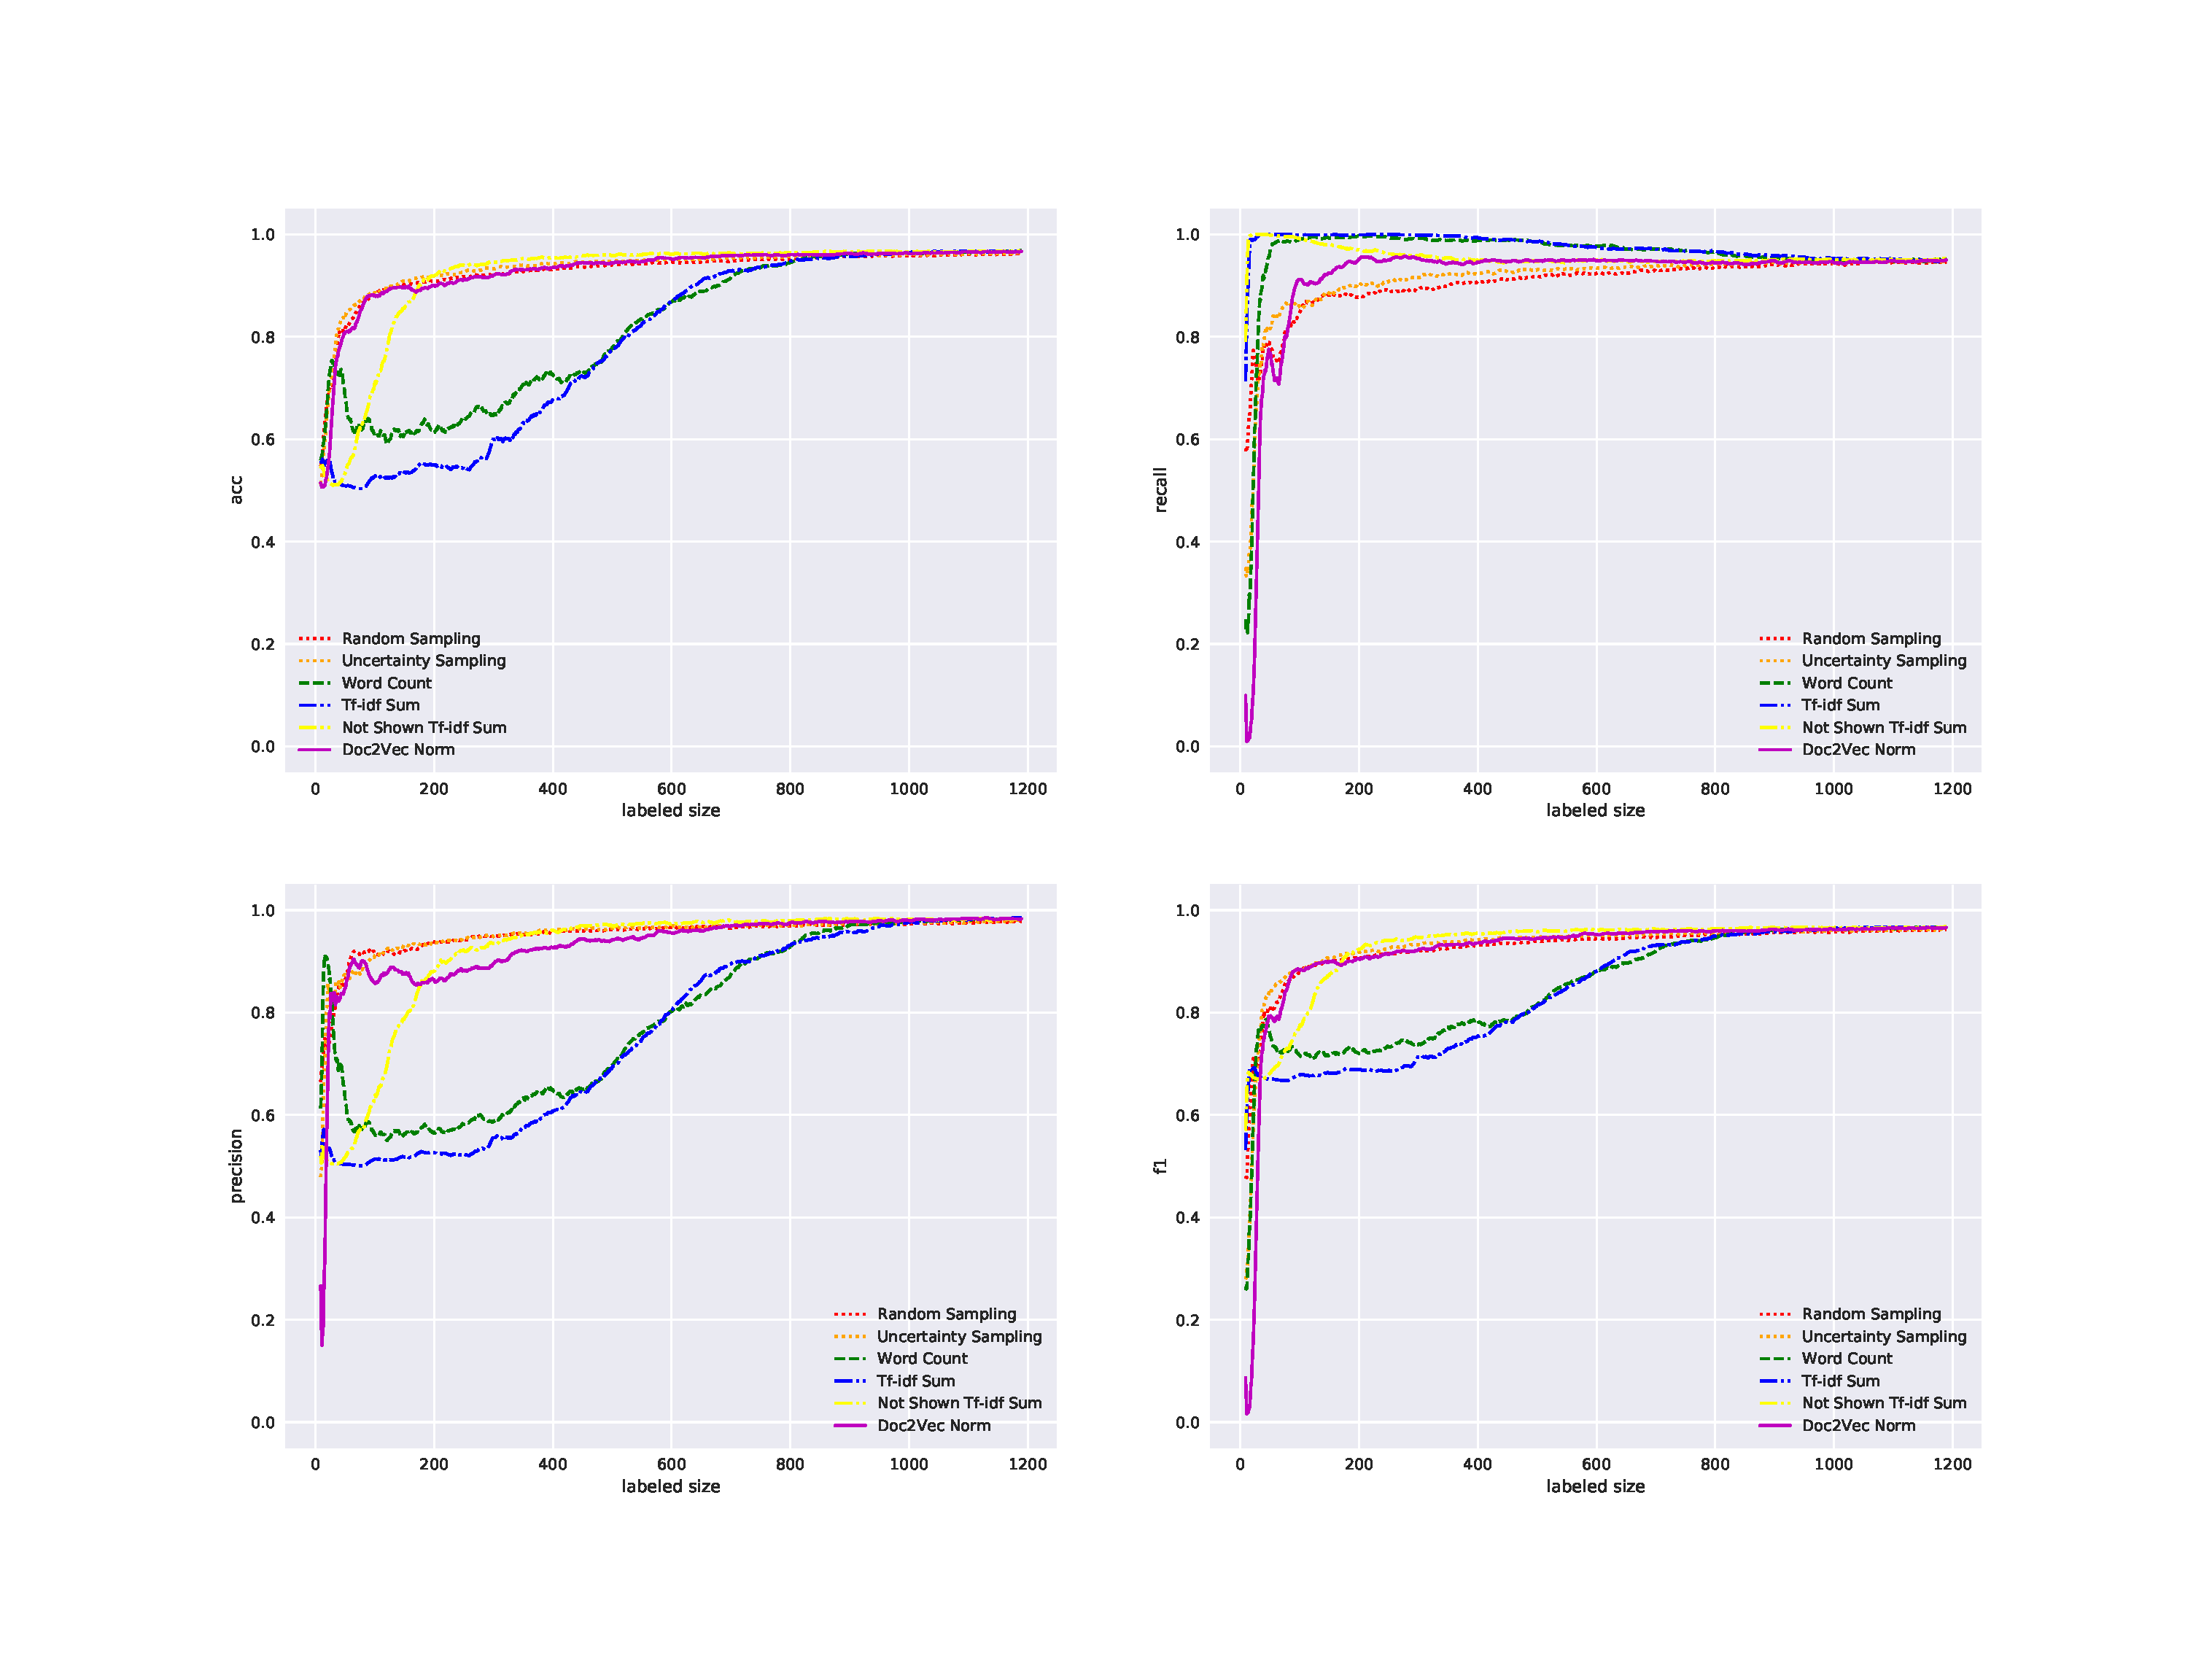
\includegraphics[width=\textwidth]{img/sms_spam_50/performance-base.eps}
\captionof{figure}{Performance of Base Approaches on Oracle Test Data of Dataset 1}
\label{performance-base1}
\end{figure}

\begin{figure}[!t]
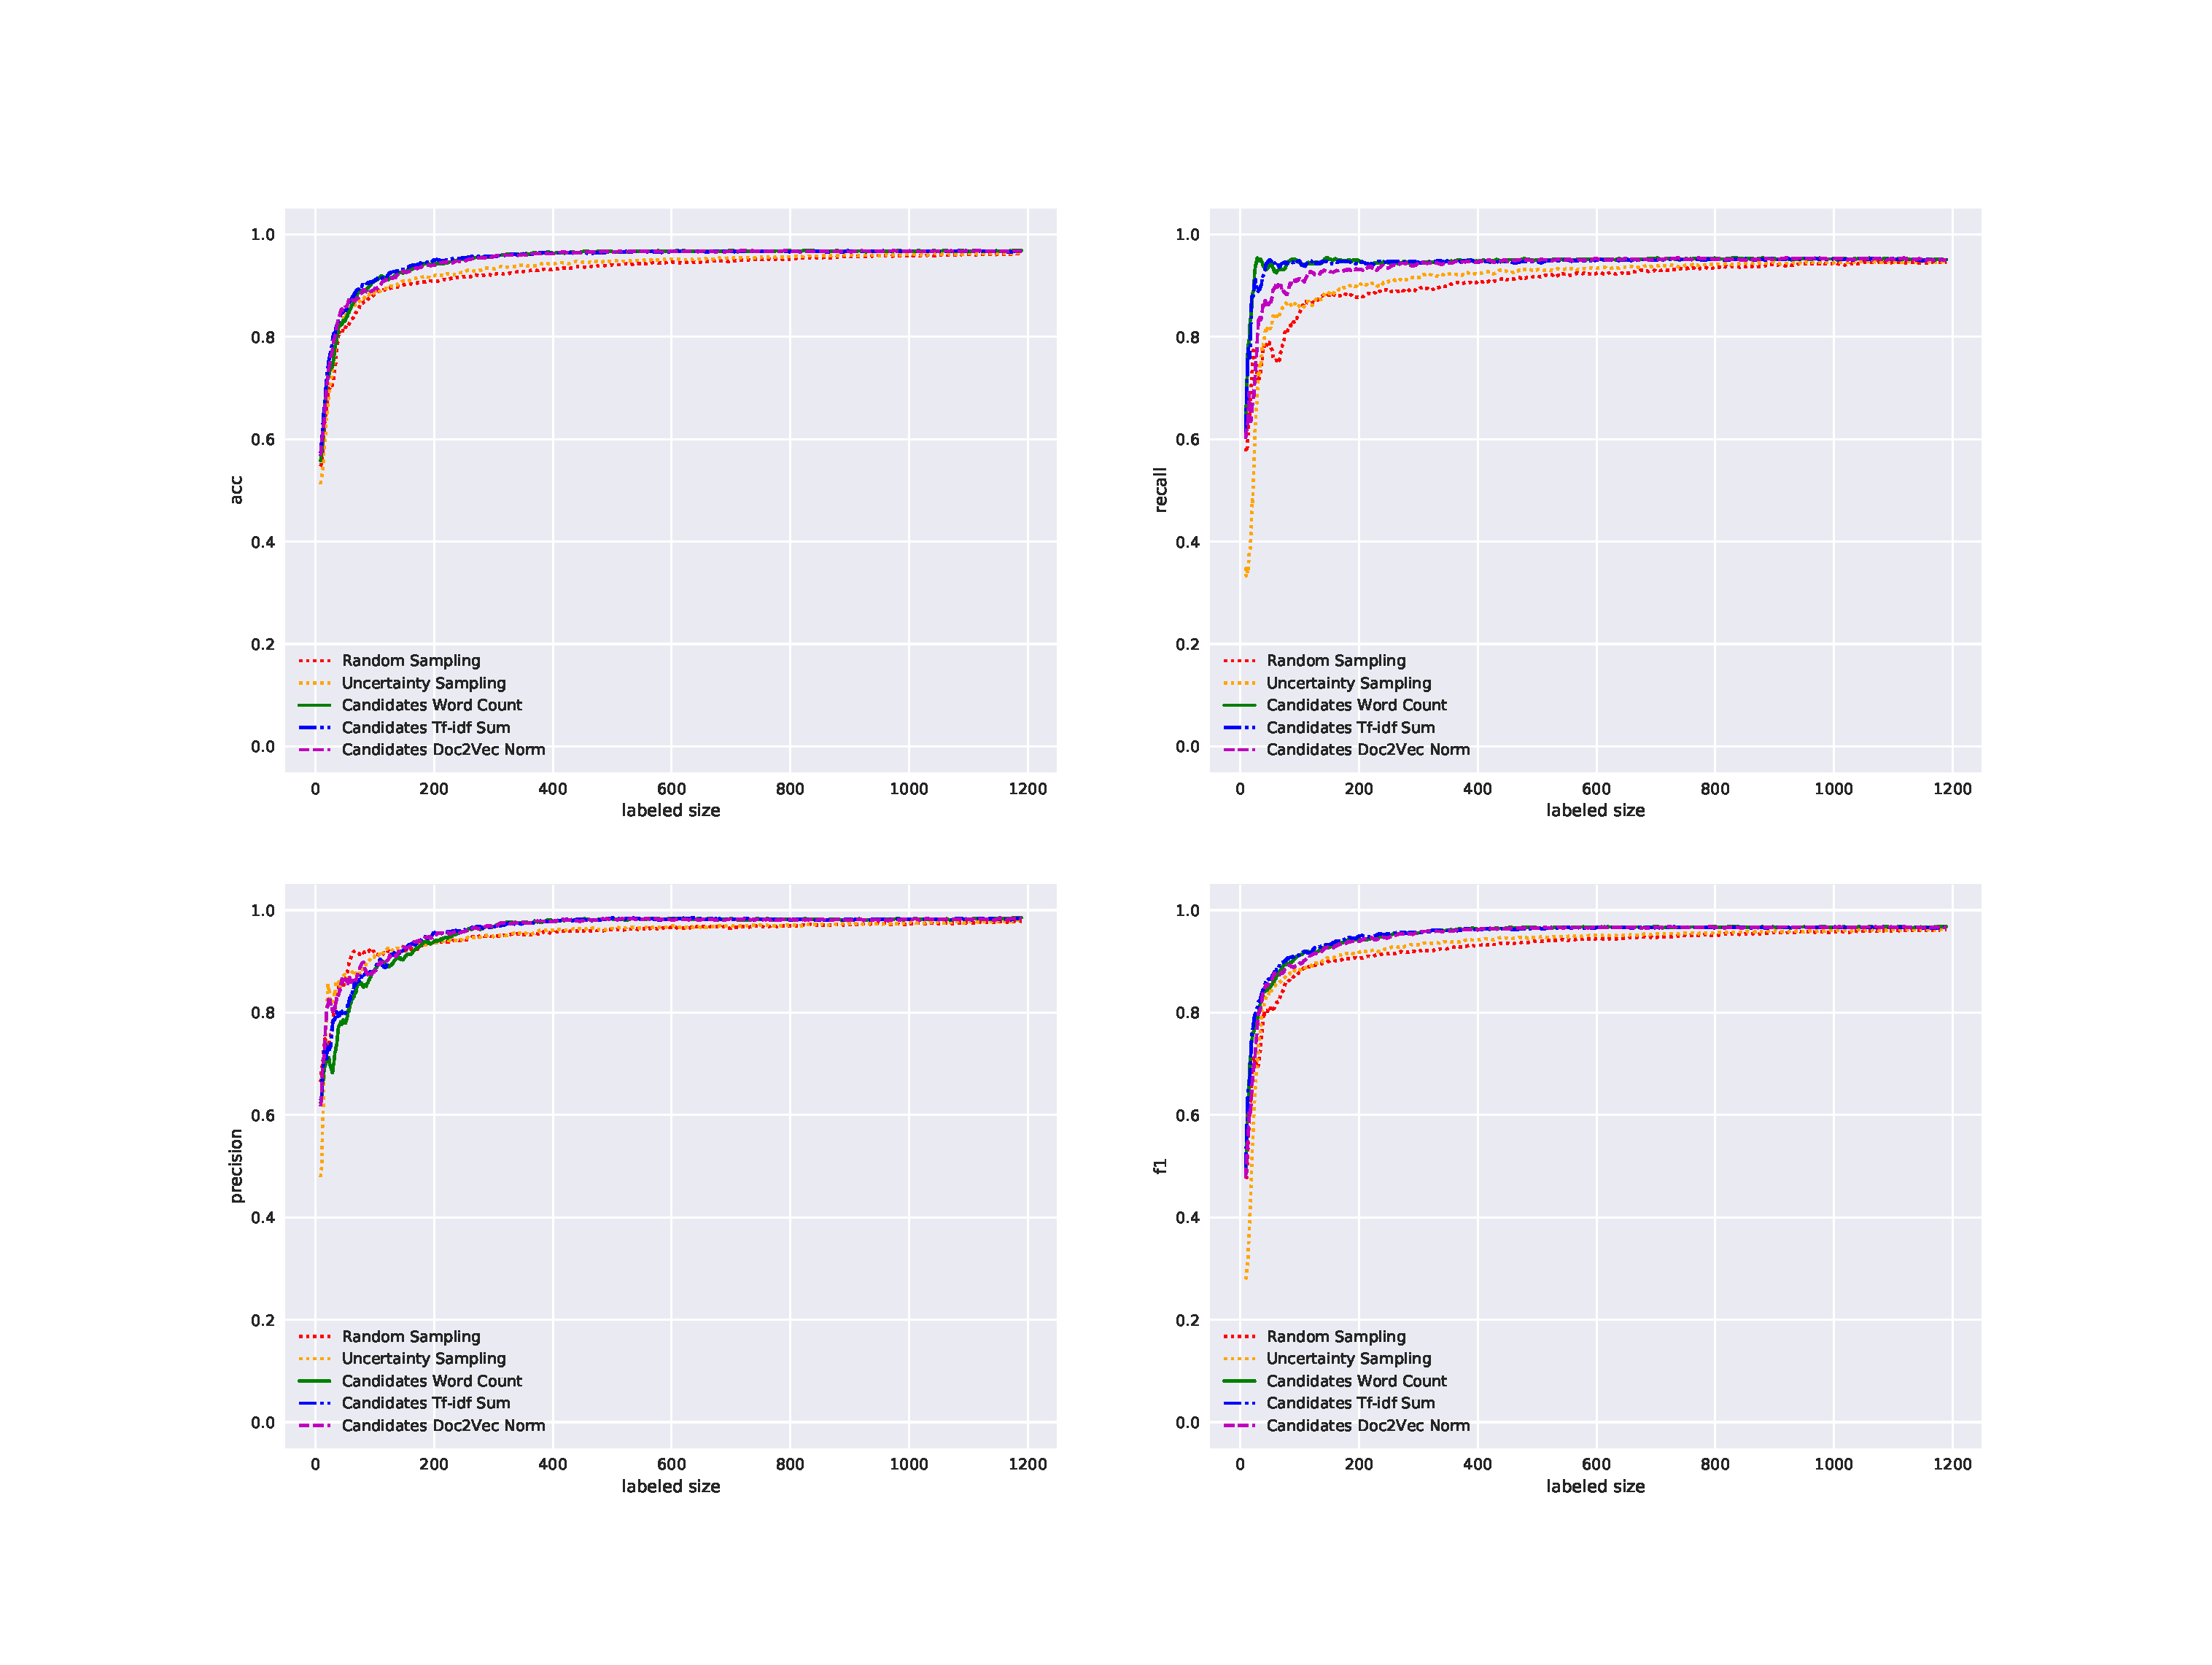
\includegraphics[width=\textwidth]{img/sms_spam_50/performance-combine.eps}
\captionof{figure}{Performance of Combination Approaches on Oracle Test Data of Dataset 1}
\label{performance-combine1}
\end{figure}

\begin{figure}[!t]
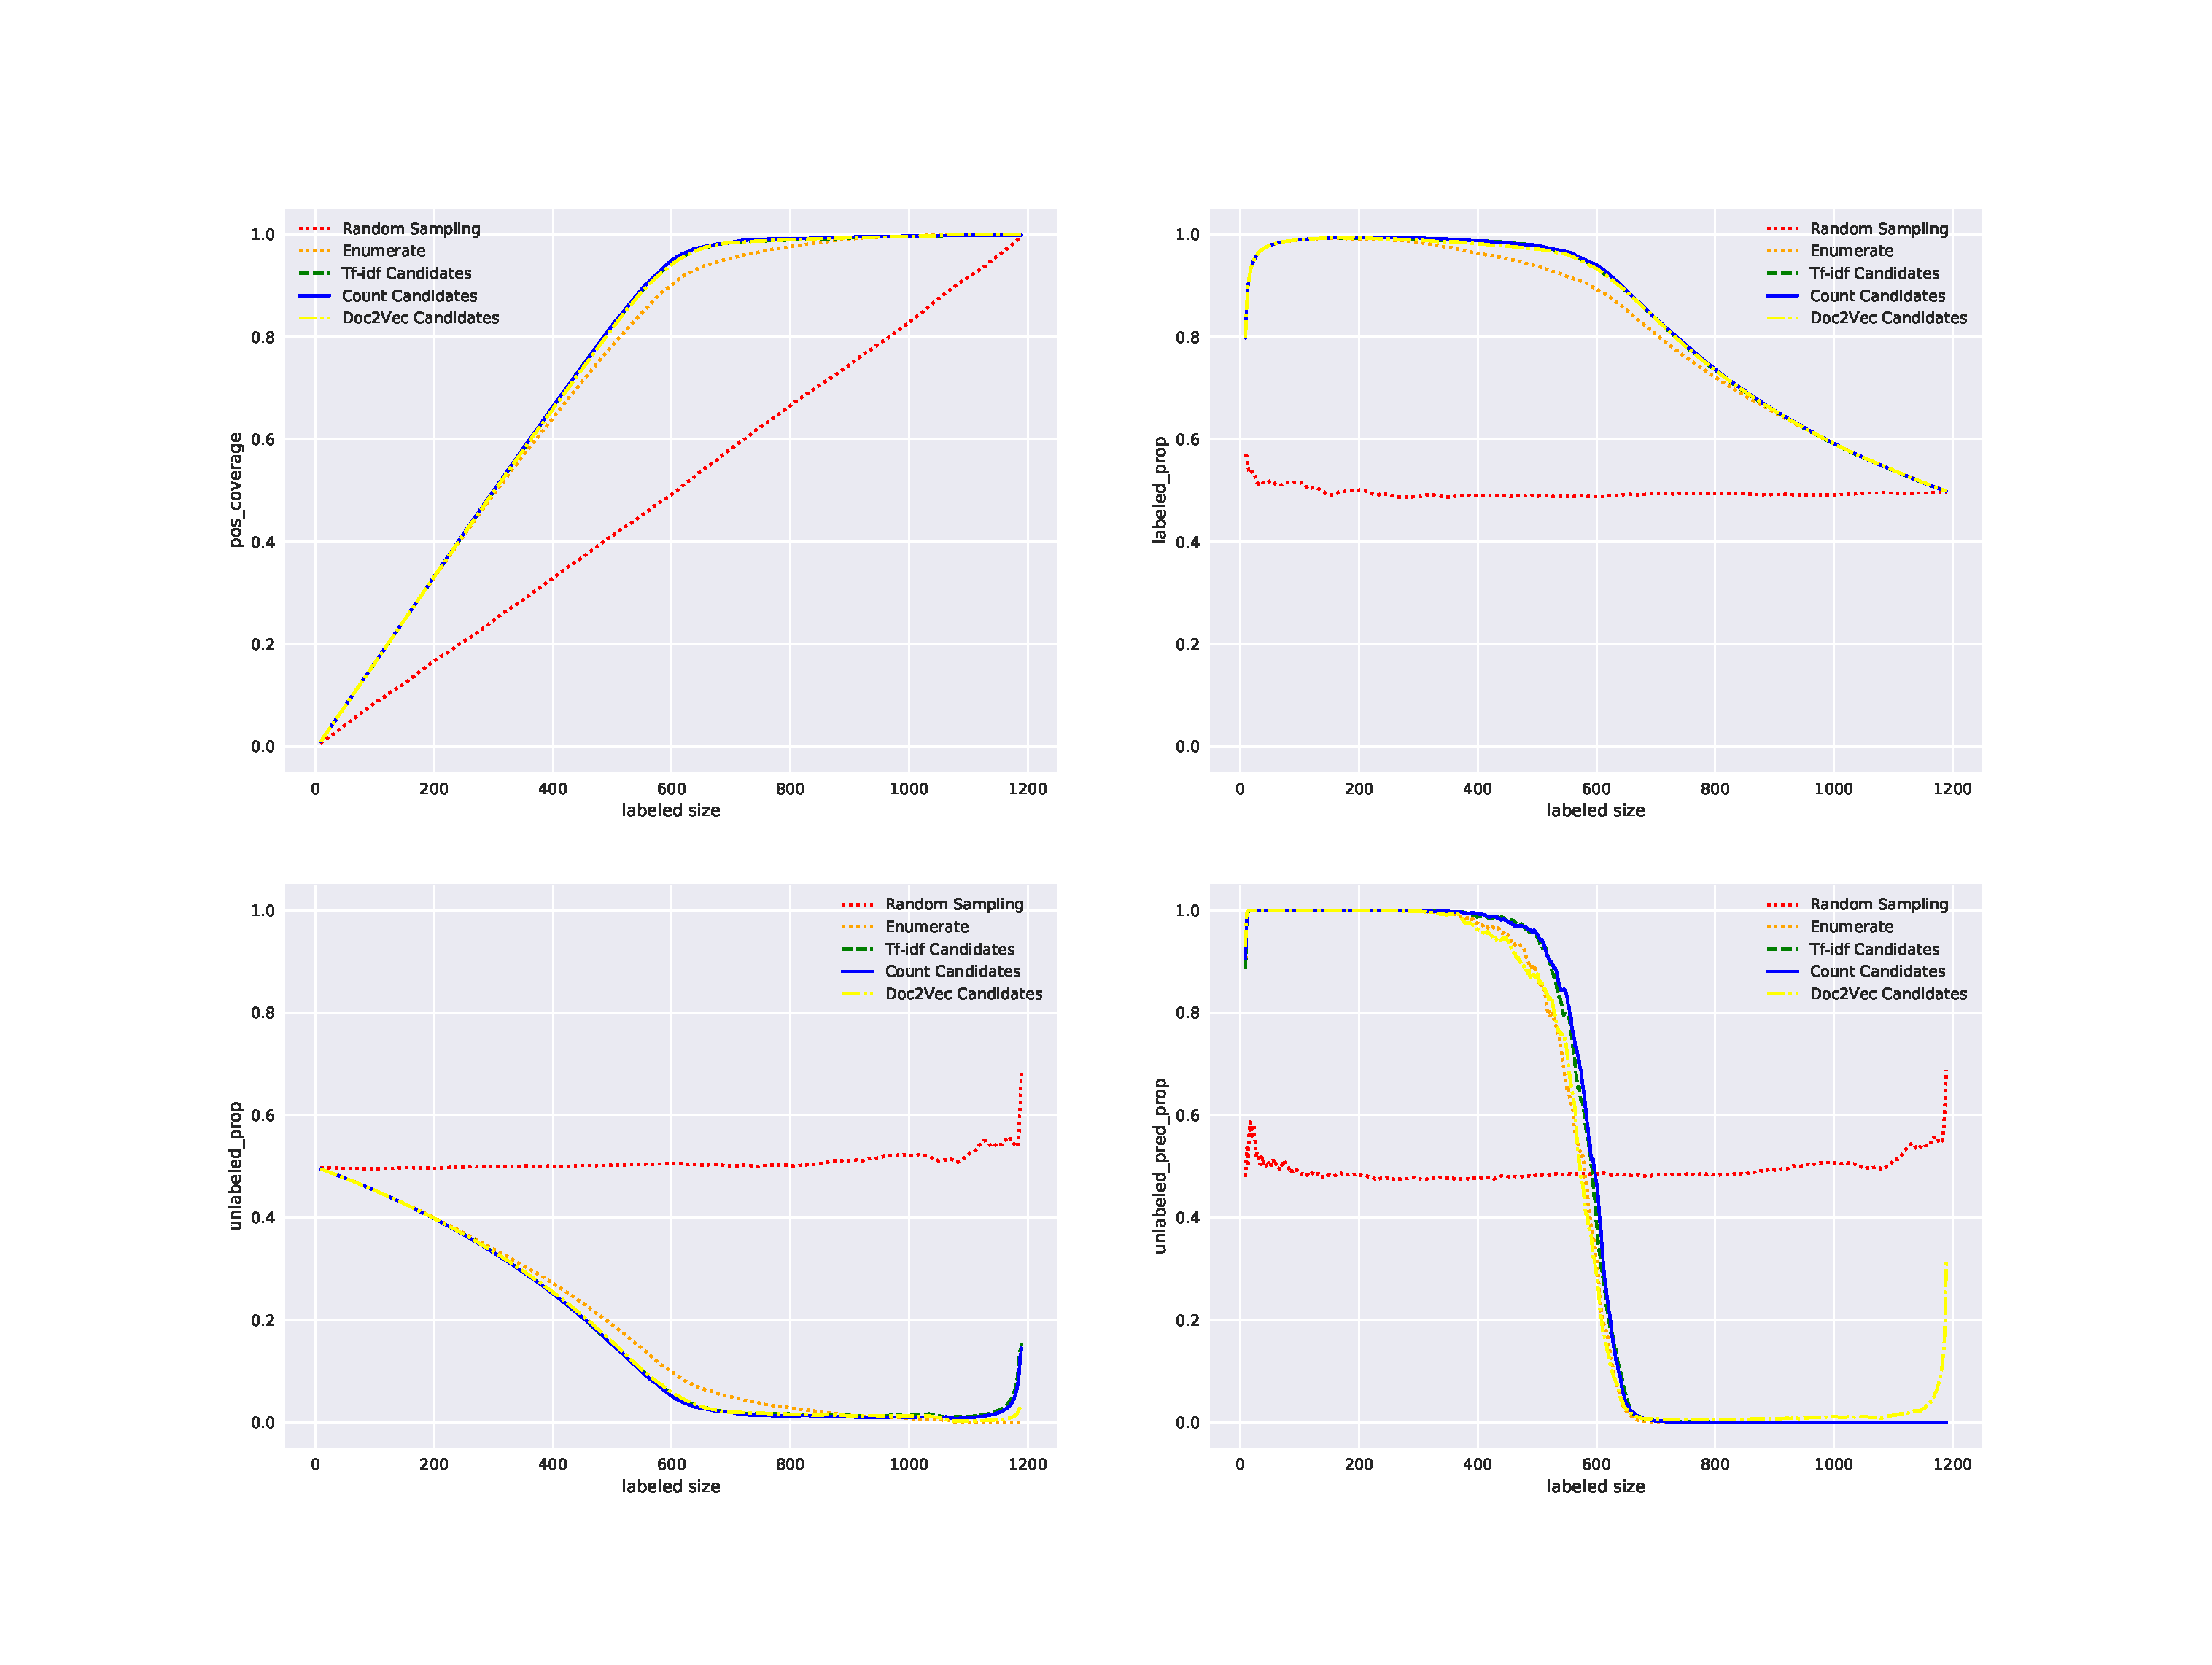
\includegraphics[width=\textwidth]{img/sms_spam_50/enumerate.eps}
\captionof{figure}{Target Retrieval on Dataset 1}
\label{enumerate1}
\end{figure}

\begin{figure}[!t]
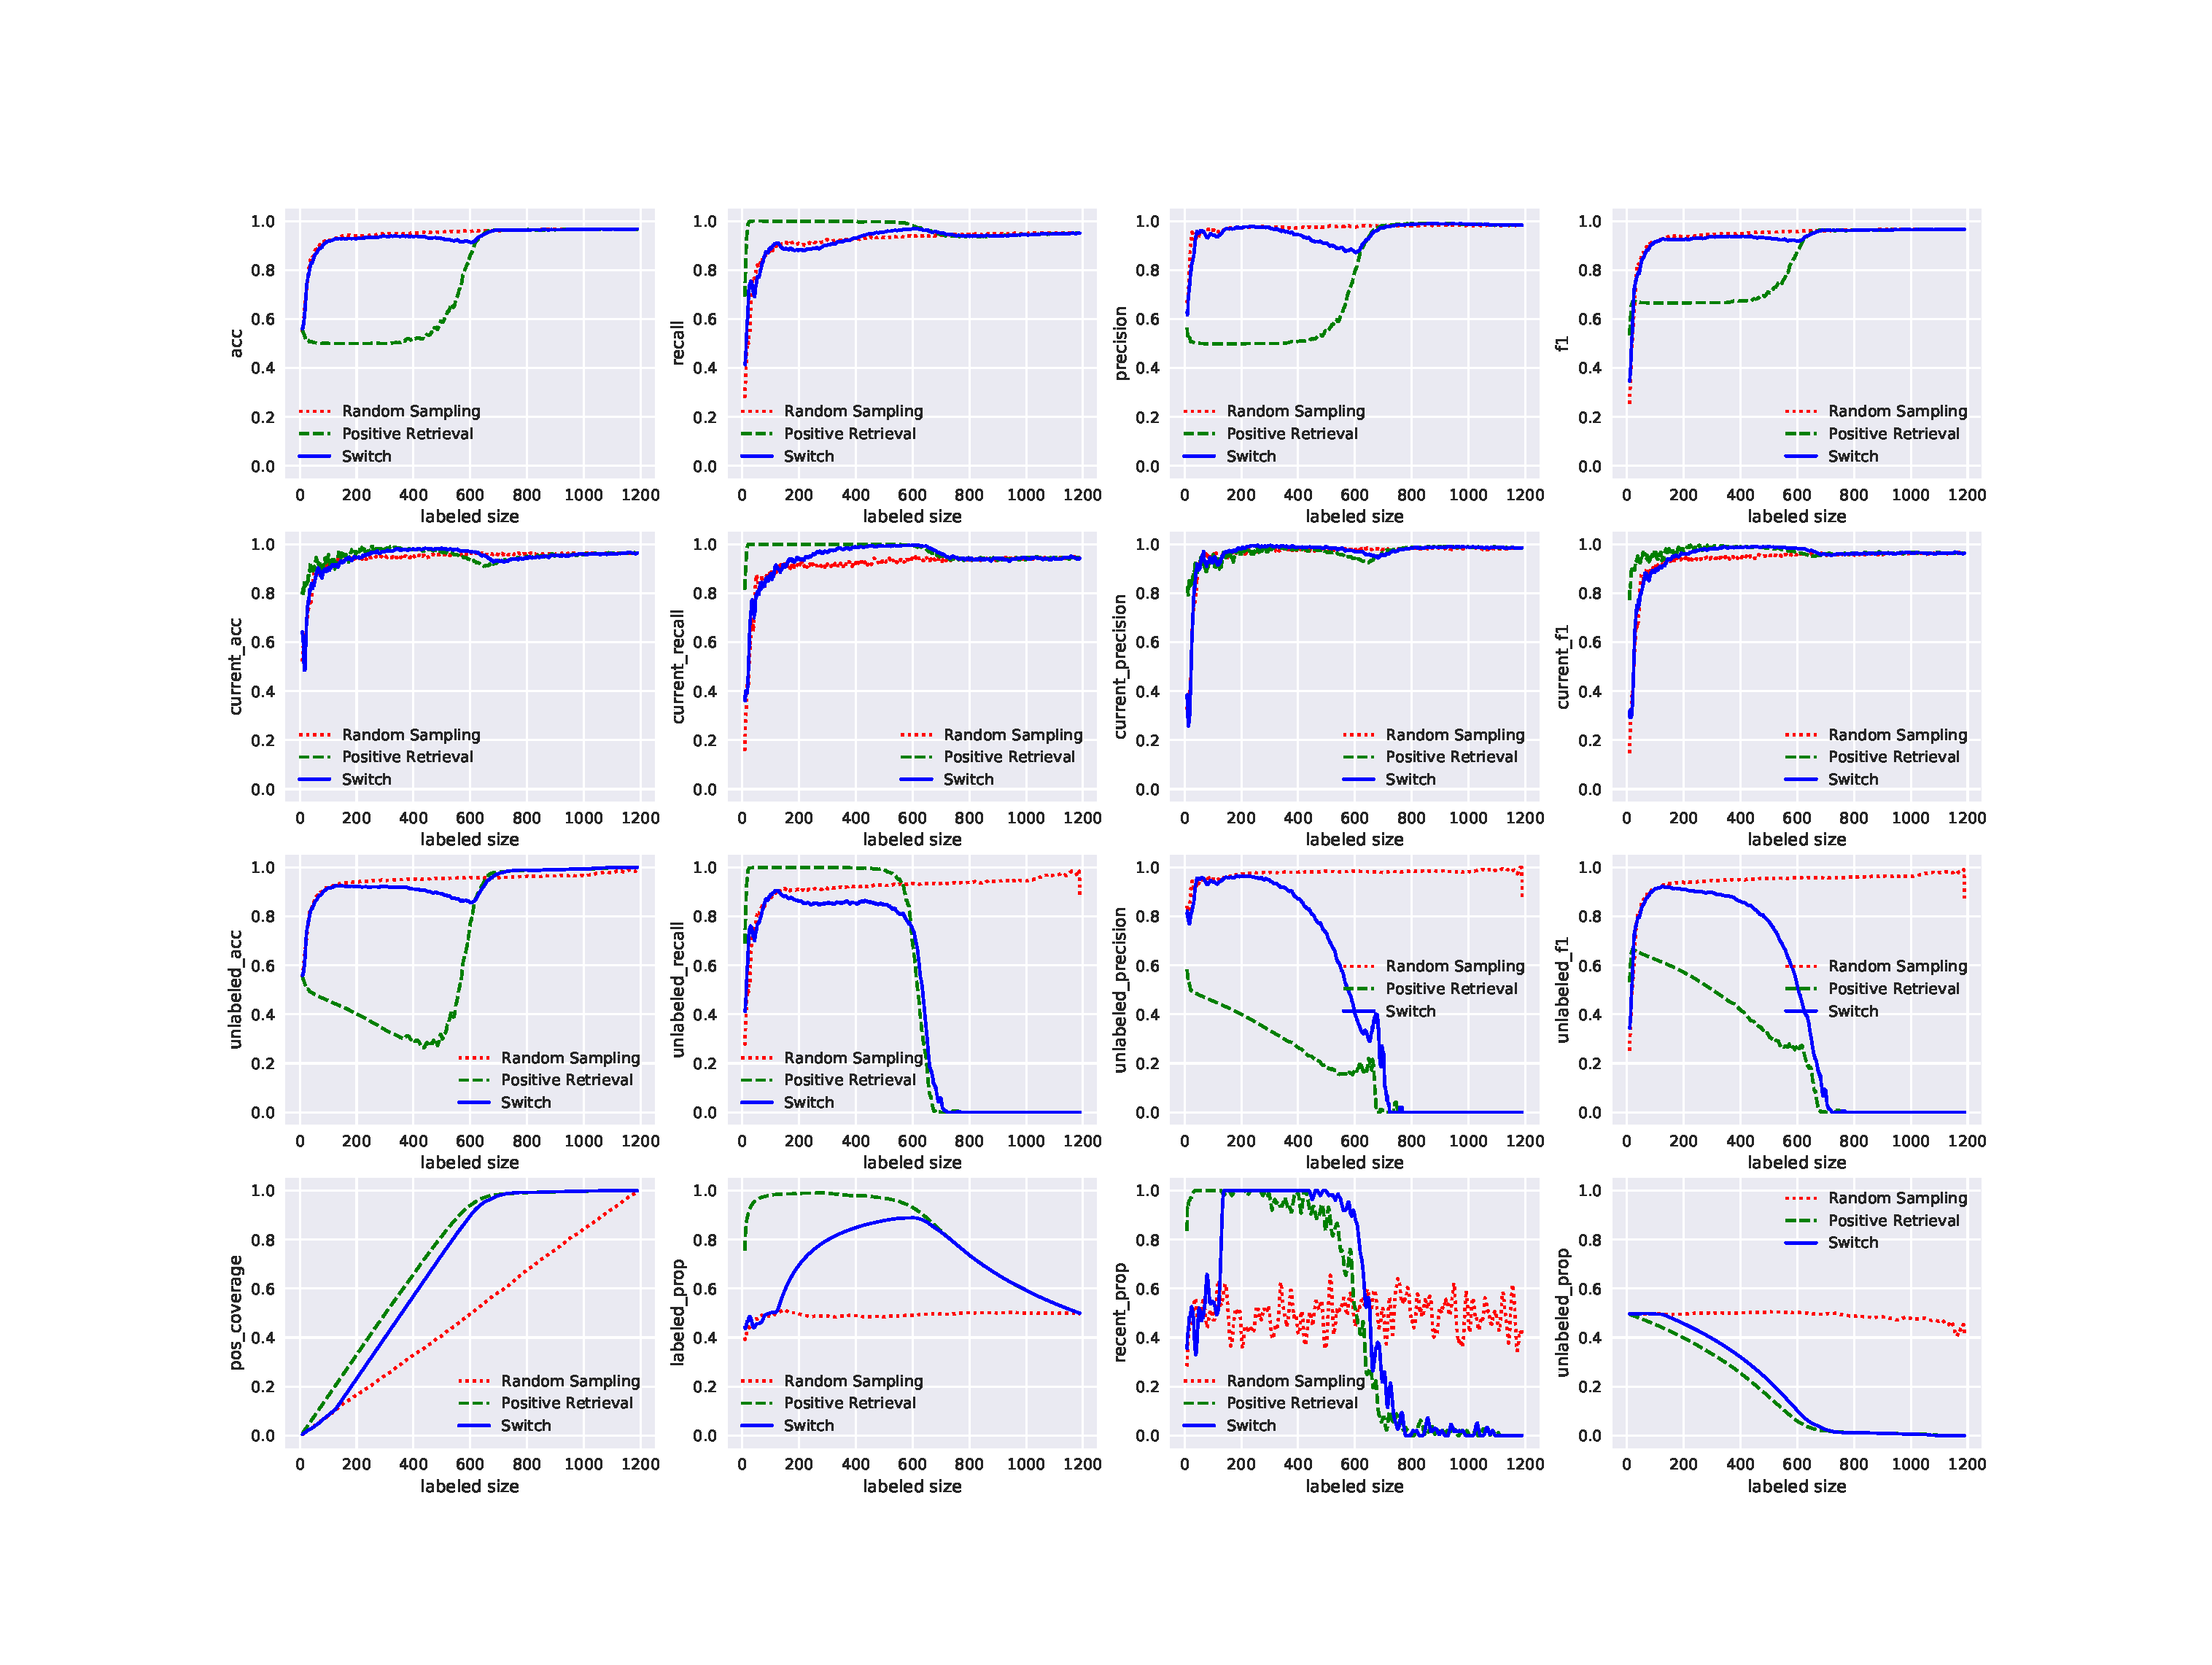
\includegraphics[width=\textwidth]{img/sms_spam_50/metrics.eps}
\captionof{figure}{Metrics on Dataset 1}
\label{metrics1}
\end{figure}

\begin{figure}[!t]
\centering
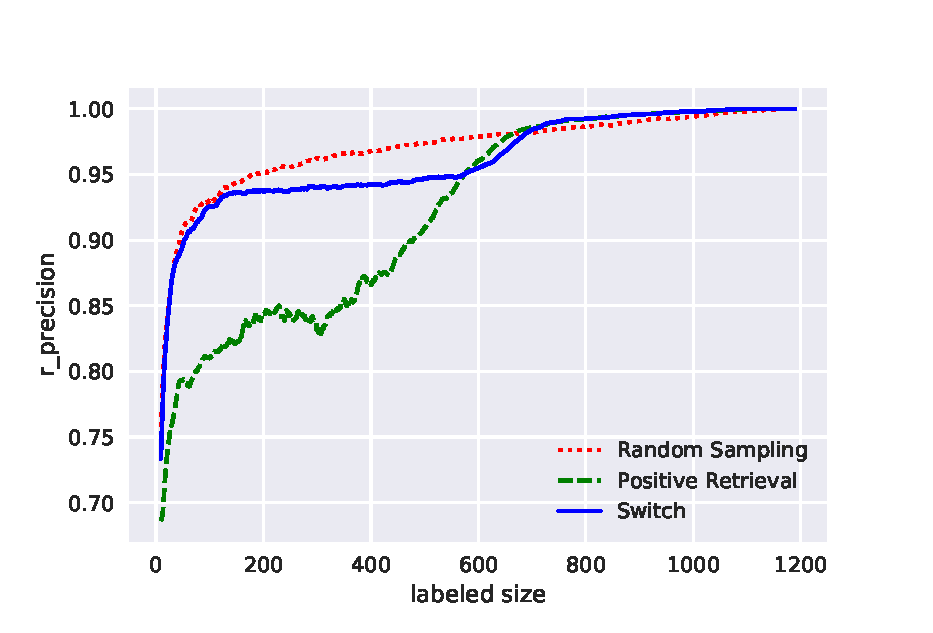
\includegraphics[width=0.6\textwidth]{img/sms_spam_50/rprecision.eps}
\captionof{figure}{R-Precision on Dataset 1}
\label{rprecision1}
\end{figure}

\begin{figure}[!t]
\includegraphics[width=\textwidth]{img/sms_spam_50/heat_map.eps}
\captionof{figure}{Heat Map on Dataset 1}
\label{heatmap1}
\end{figure}

\begin{figure}[!t]
\includegraphics[width=\textwidth]{img/sms_spam_50/true_heat_map.eps}
\captionof{figure}{Heat Map of True Layer on Dataset 1}
\label{true_heatmap1}
\end{figure}

\begin{figure}[!t]
\includegraphics[width=\textwidth]{img/sms_spam_50/false_heat_map.eps}
\captionof{figure}{Heat Map of False Layer on Dataset 1}
\label{false_heatmap1}
\end{figure}

I will discuss the experimental results on Dataset 1 separately according to my three purpose.

\subsubsection{Improving the Performance of Obtained Model}
Figure \ref{performance-base1} and \ref{performance-combine1} show the performance of base methods and combination methods on oracle test set. I can find out that base methods of unique word count, tf-idf summation and Tf-idf summation of words not shown give poor f1-score, but show better recall than random sampling and uncertainty sampling baseline, while Doc2Vec norm method shows a same level performance compared to the two baselines. As for the combination methods, all proposed methods give a little but obvious better performance than the two baselines, especially on the metric of recall.

\subsubsection{Finding Data from Target Class Faster}
Figure \ref{enumerate1} shows metrics to measure how fast the model find target data. From positive coverage, I can find out that random sampling baseline gives a linear result, while learning-to-enumerate baseline gives a much better performance than random sampling. My proposed methods gives a little but obvious better results, while differences among proposed methods are subtle.

\subsubsection{Tackling the Performance-Target Dilemma}
In Figure \ref{metrics1} (Row 4, Column 1), from positive coverage, I can find out that target-retrieval-learning works expectedly. Also, in Figure \ref{metrics1} (Row 1), since both accuracy and f1-score on oracle test set show good result at final step, I can assert that the model is well trained. However, random sampling gives a much better learning speed (Row 1, Column 4, f1-score) than target-retrieval-learning, since the labeled data does not have any bias. While in target-retrieval-learning, the model does not learn well at the early phase, since the labeled data used to train is biased towards target samples, which can be known from target proportion in unlabeled data (Row 4, Column 4). As the model find most of target samples, non-target samples begin to increase in the labeled data, so that the model can start to learn the classification task properly. In current test set, there is an obvious pit in accuracy, precision and f1-score. The reason is that, at the early phase, the current test set is also biased, even thought the model does not well learned, I cannot know it from the current test set metrics. At the later phase, as the current test set gradually becomes balanced, these metrics begin to go down. when the model begin to learn the classification task, metrics go up again.

From the aspect of R-precision, I can see from Figure \ref{rprecision1} that in early steps, when the model is not well learned, the model shows poor R-precision comparing to random sampling. On the contrary, when the model starts to perform well from around step 600, R-precision of target-retrieval-learning goes superior than random sampling, which indicates that the model trained by target-retrieval-learning algorithm also provides a better ranking. This satisfies my second purpose of providing a target likelihood ranking, so that I can switch to model prediction from human annotation. Also I can see that although the AUC of R-precision of switch method do not surpass random sampling, but gives much better performance than target retrieval method.

In recent labeled target proportion (Figure \ref{metrics1}--Row 4), it indicates the proportion of target sample in the recent ten labeled data. Random sampling shows a relatively stable curve as expected, while target-retrieval-learning picks much more target samples at early steps, but as target samples remaining less in unlabeled data, the proportion goes low at later steps. Since this is a metric which can be known in real application, it provide a possibility to estimate the target proportion of unlabeled data. Also, if I do a few random sampling at the very start of annotation process, it will provide a priori of the whole unlabeled pool. So in switch method, which use random sampling in the start 1/10 steps, and then switch to target-retrieval method, gives a little poor positive coverage at the early phase, but in exchange, I am able to have a estimation about the distribution of the whole dataset from the random sampling part (Row 4, Column 3). I can see that at the early phase of switch method, the curve overlaps with random sampling, this gives us information about the priori of the unlabeled pool.

The head map is the histogram of normalize distance to the decision boundary with current model of unlabeled samples. I consider this normalized distance as an approximate likelihood, although distance is different from possibility. From Figure \ref{heatmap1}, I can find out that in random sampling, since the model is well trained, there are two obvious clusters representing target and non-target. As for target-retrieval-learning, I cannot tell the difference between target and non-target. However, the strange thing is, from Figure \ref{metrics1} (Row 1), I already know that both methods finally give proper performance, so the heat map is suppose to have two cluster at the later phase. To investigate deeper, I split the heat map into target layer and non-target layer as shown in Figure \ref{true_heatmap1} and \ref{false_heatmap1}. I can see that although it is not as obvious as random sampling, there are indeed differences between target and non-target samples, target samples locate between 0.7 to 1.0, while non-target samples locate between 0.5 to 0.8. Furthermore, few target samples remaining in unlabeled data can also be one reason of the non-obviousness.

\subsection{Dataset 2}
To investigate any influence by the unbalance of data, this time I simulate on unbalanced dataset. Similar to experiments on Dataset 1, I also discuss the results on Dataset 2 separately according to my three purpose. Figure \ref{performance-base1} and \ref{performance-combine1} show the performance of base methods and combination methods on oracle test set. 

\begin{figure}[!t]
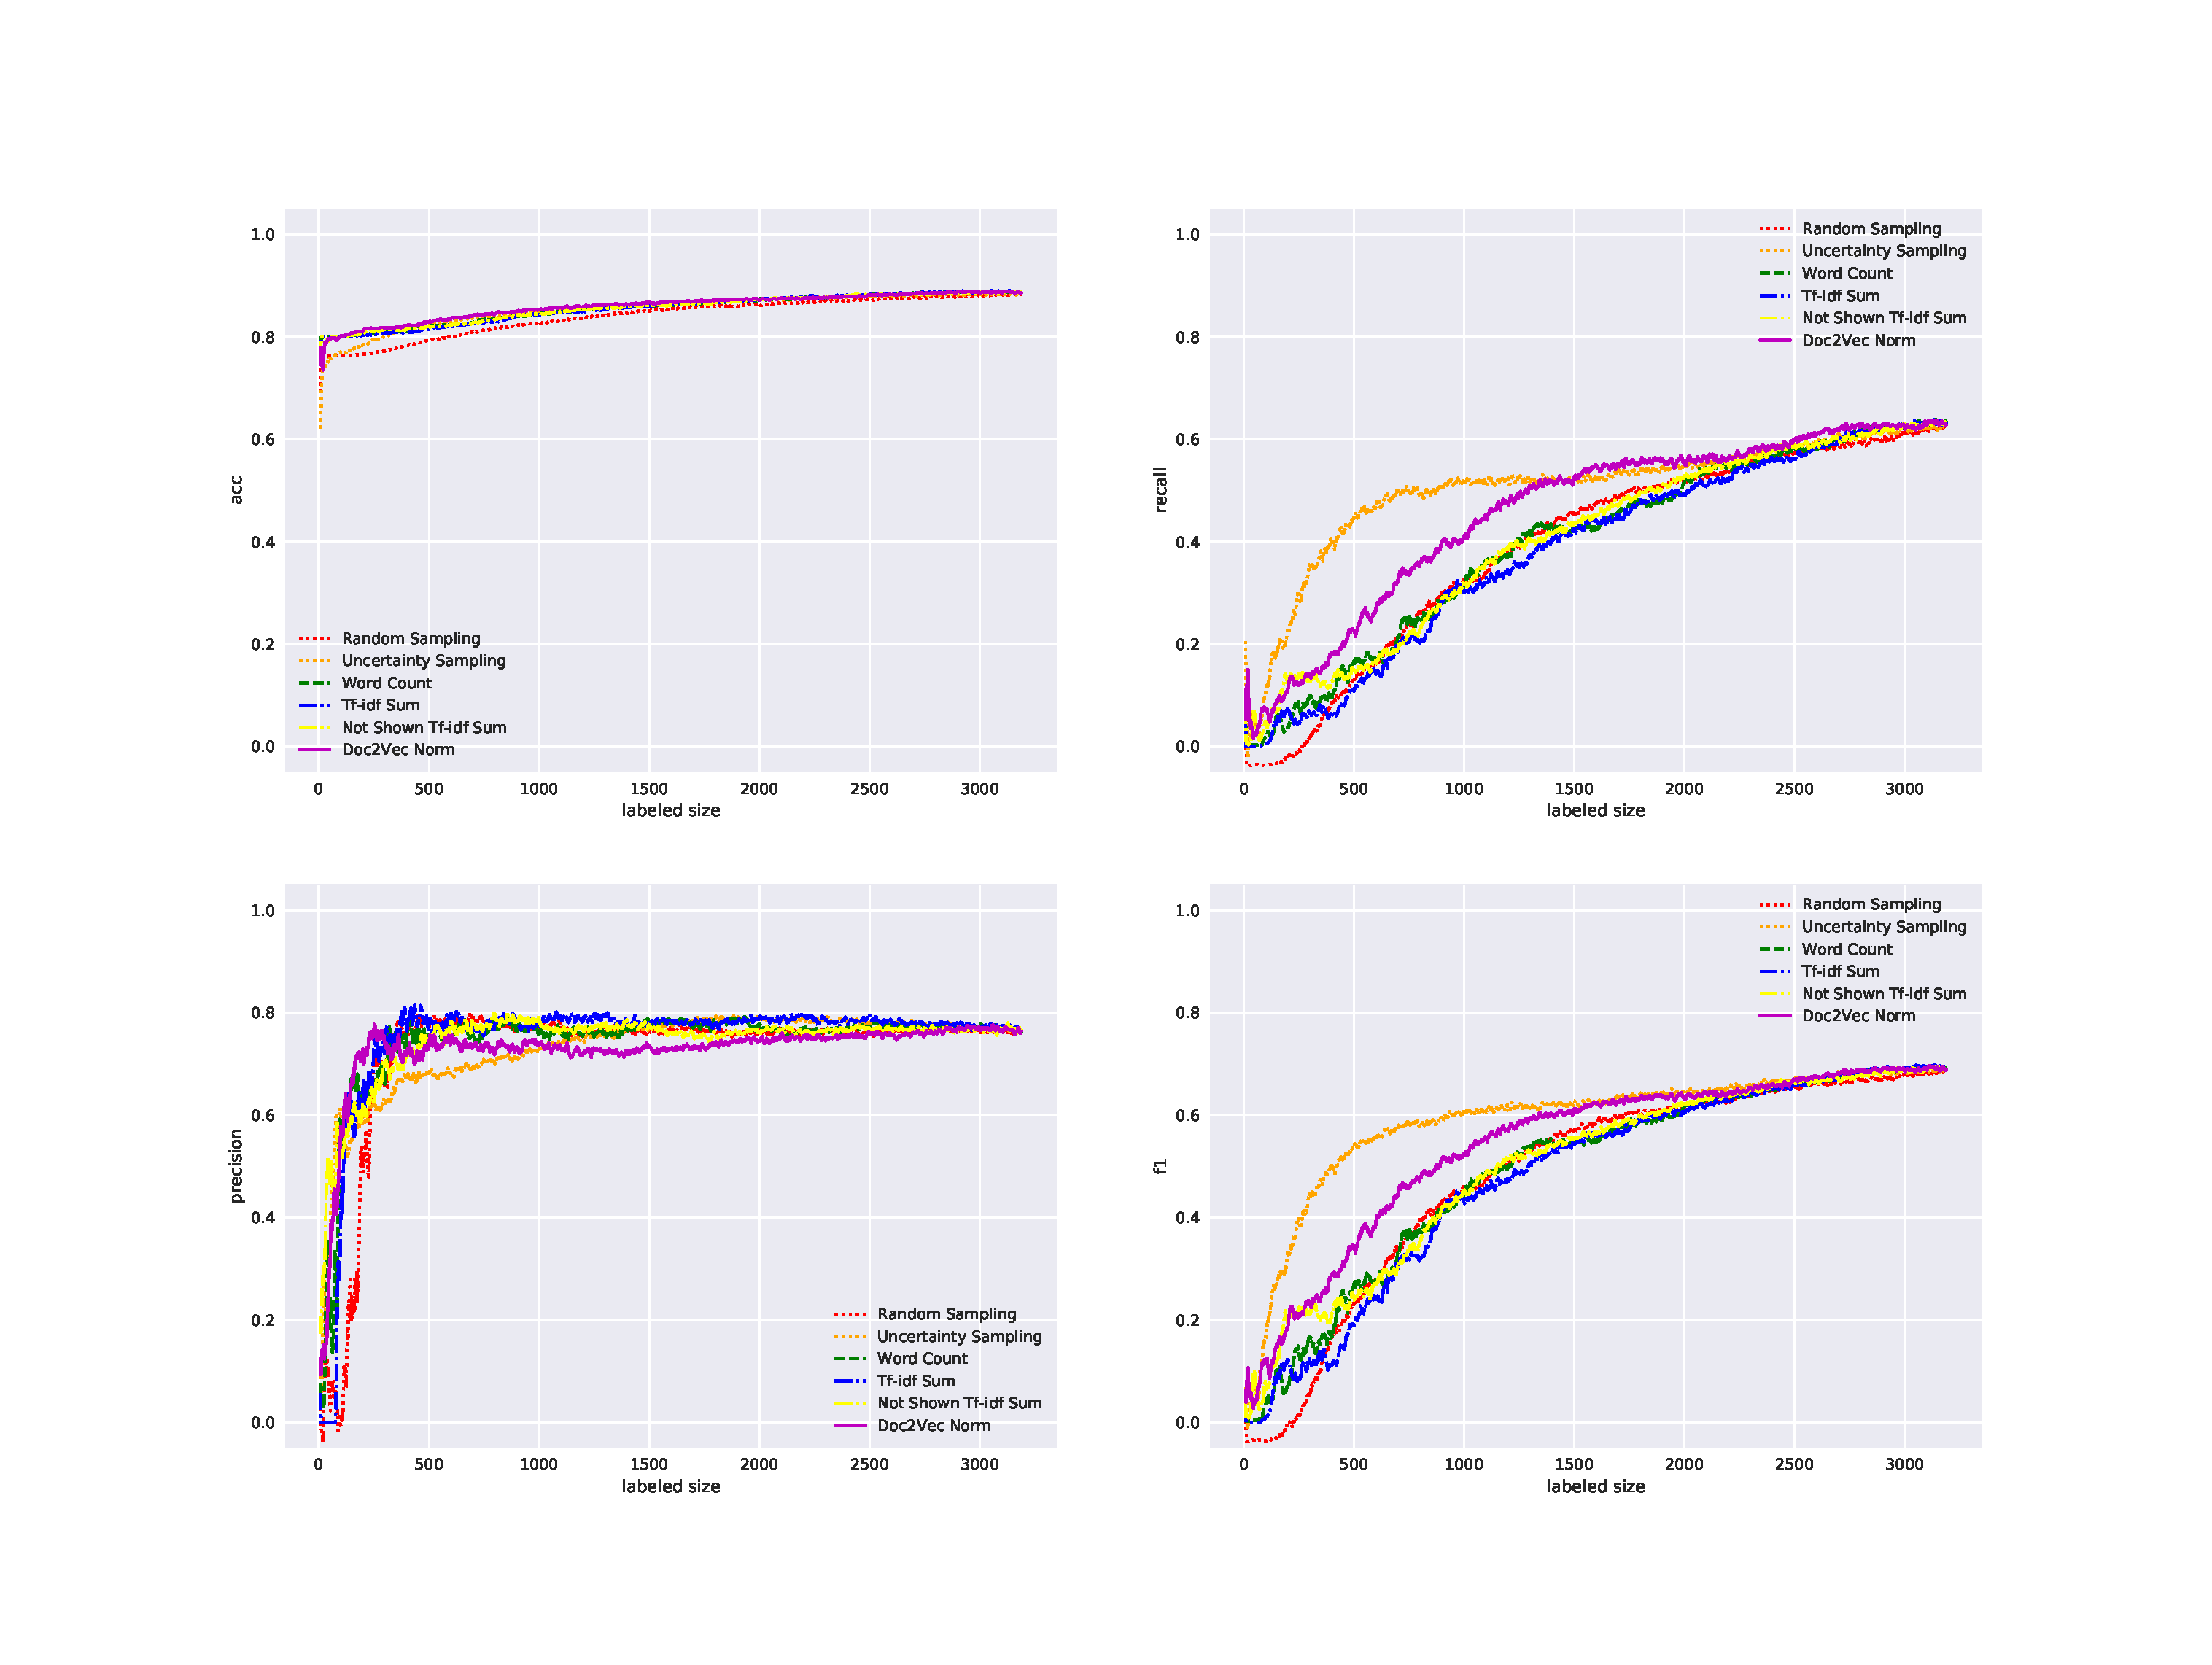
\includegraphics[width=\textwidth]{img/imdb_20/performance-base.eps}
\captionof{figure}{Performance of Base Approaches on Oracle Test Data of Dataset 2}
\label{performance-base2}
\end{figure}

\begin{figure}[!t]
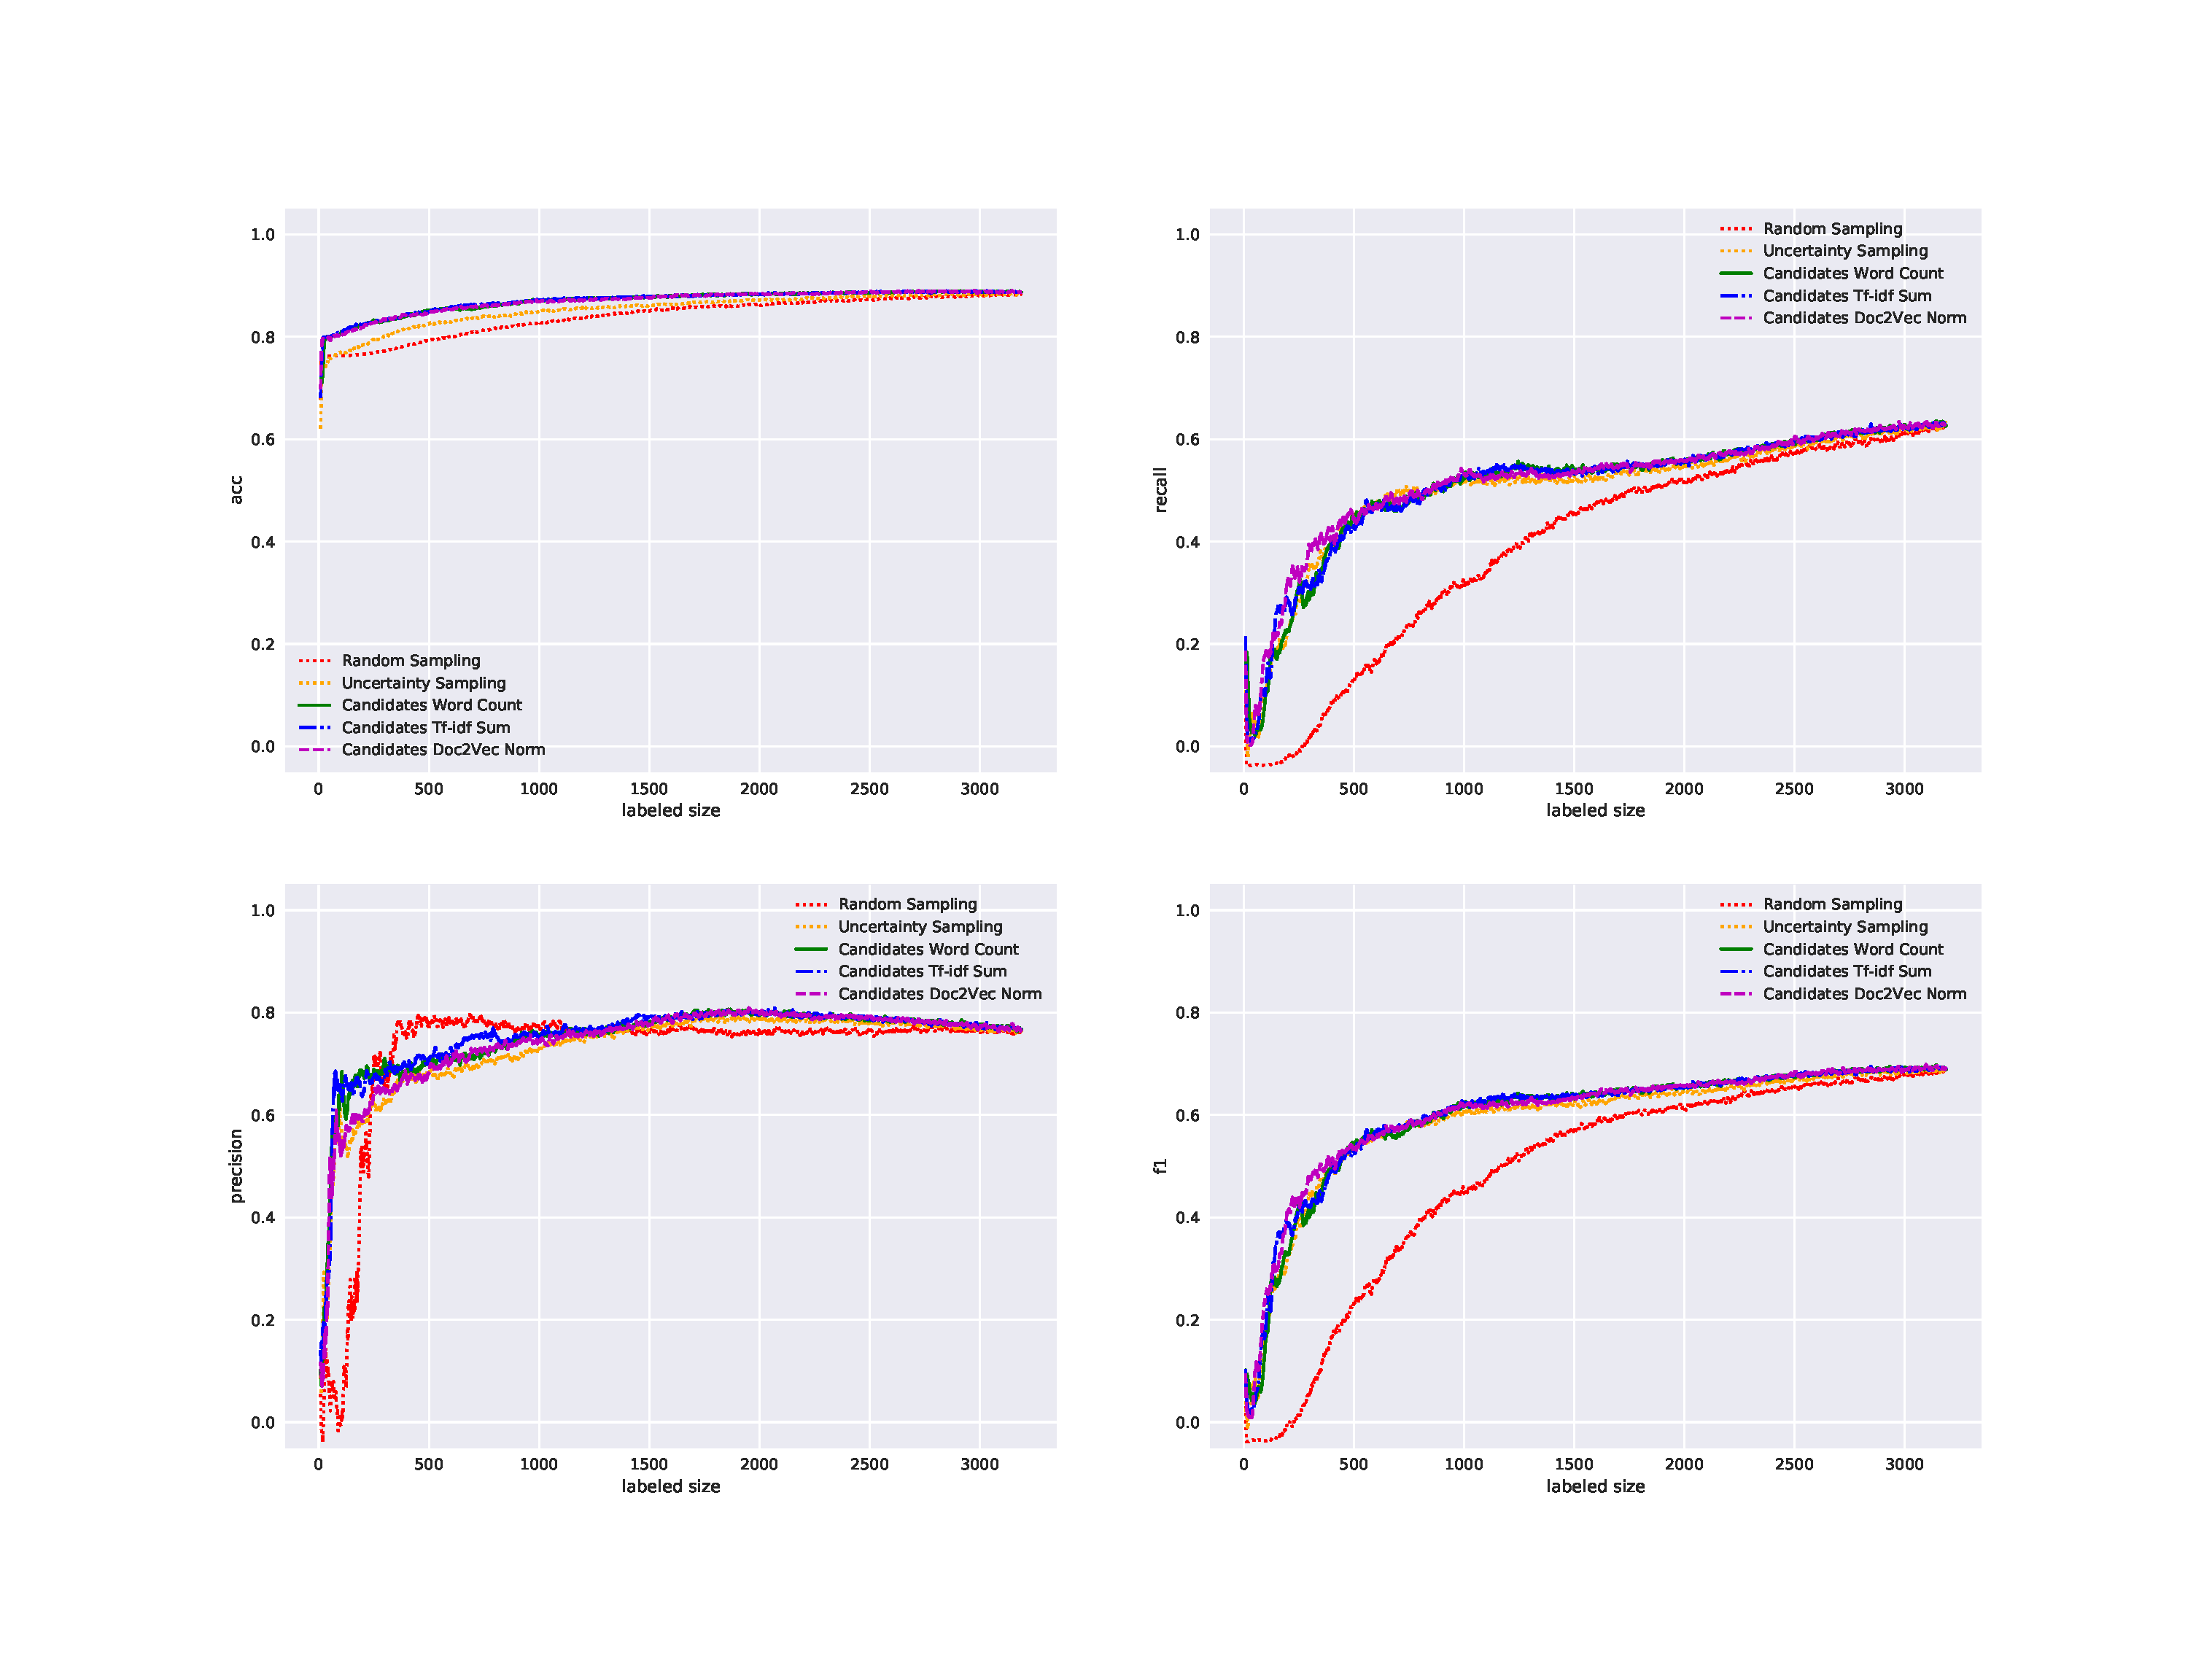
\includegraphics[width=\textwidth]{img/imdb_20/performance-combine.eps}
\captionof{figure}{Performance of Combination Approaches on Oracle Test Data of Dataset 2}
\label{performance-combine2}
\end{figure}

\begin{figure}[!t]
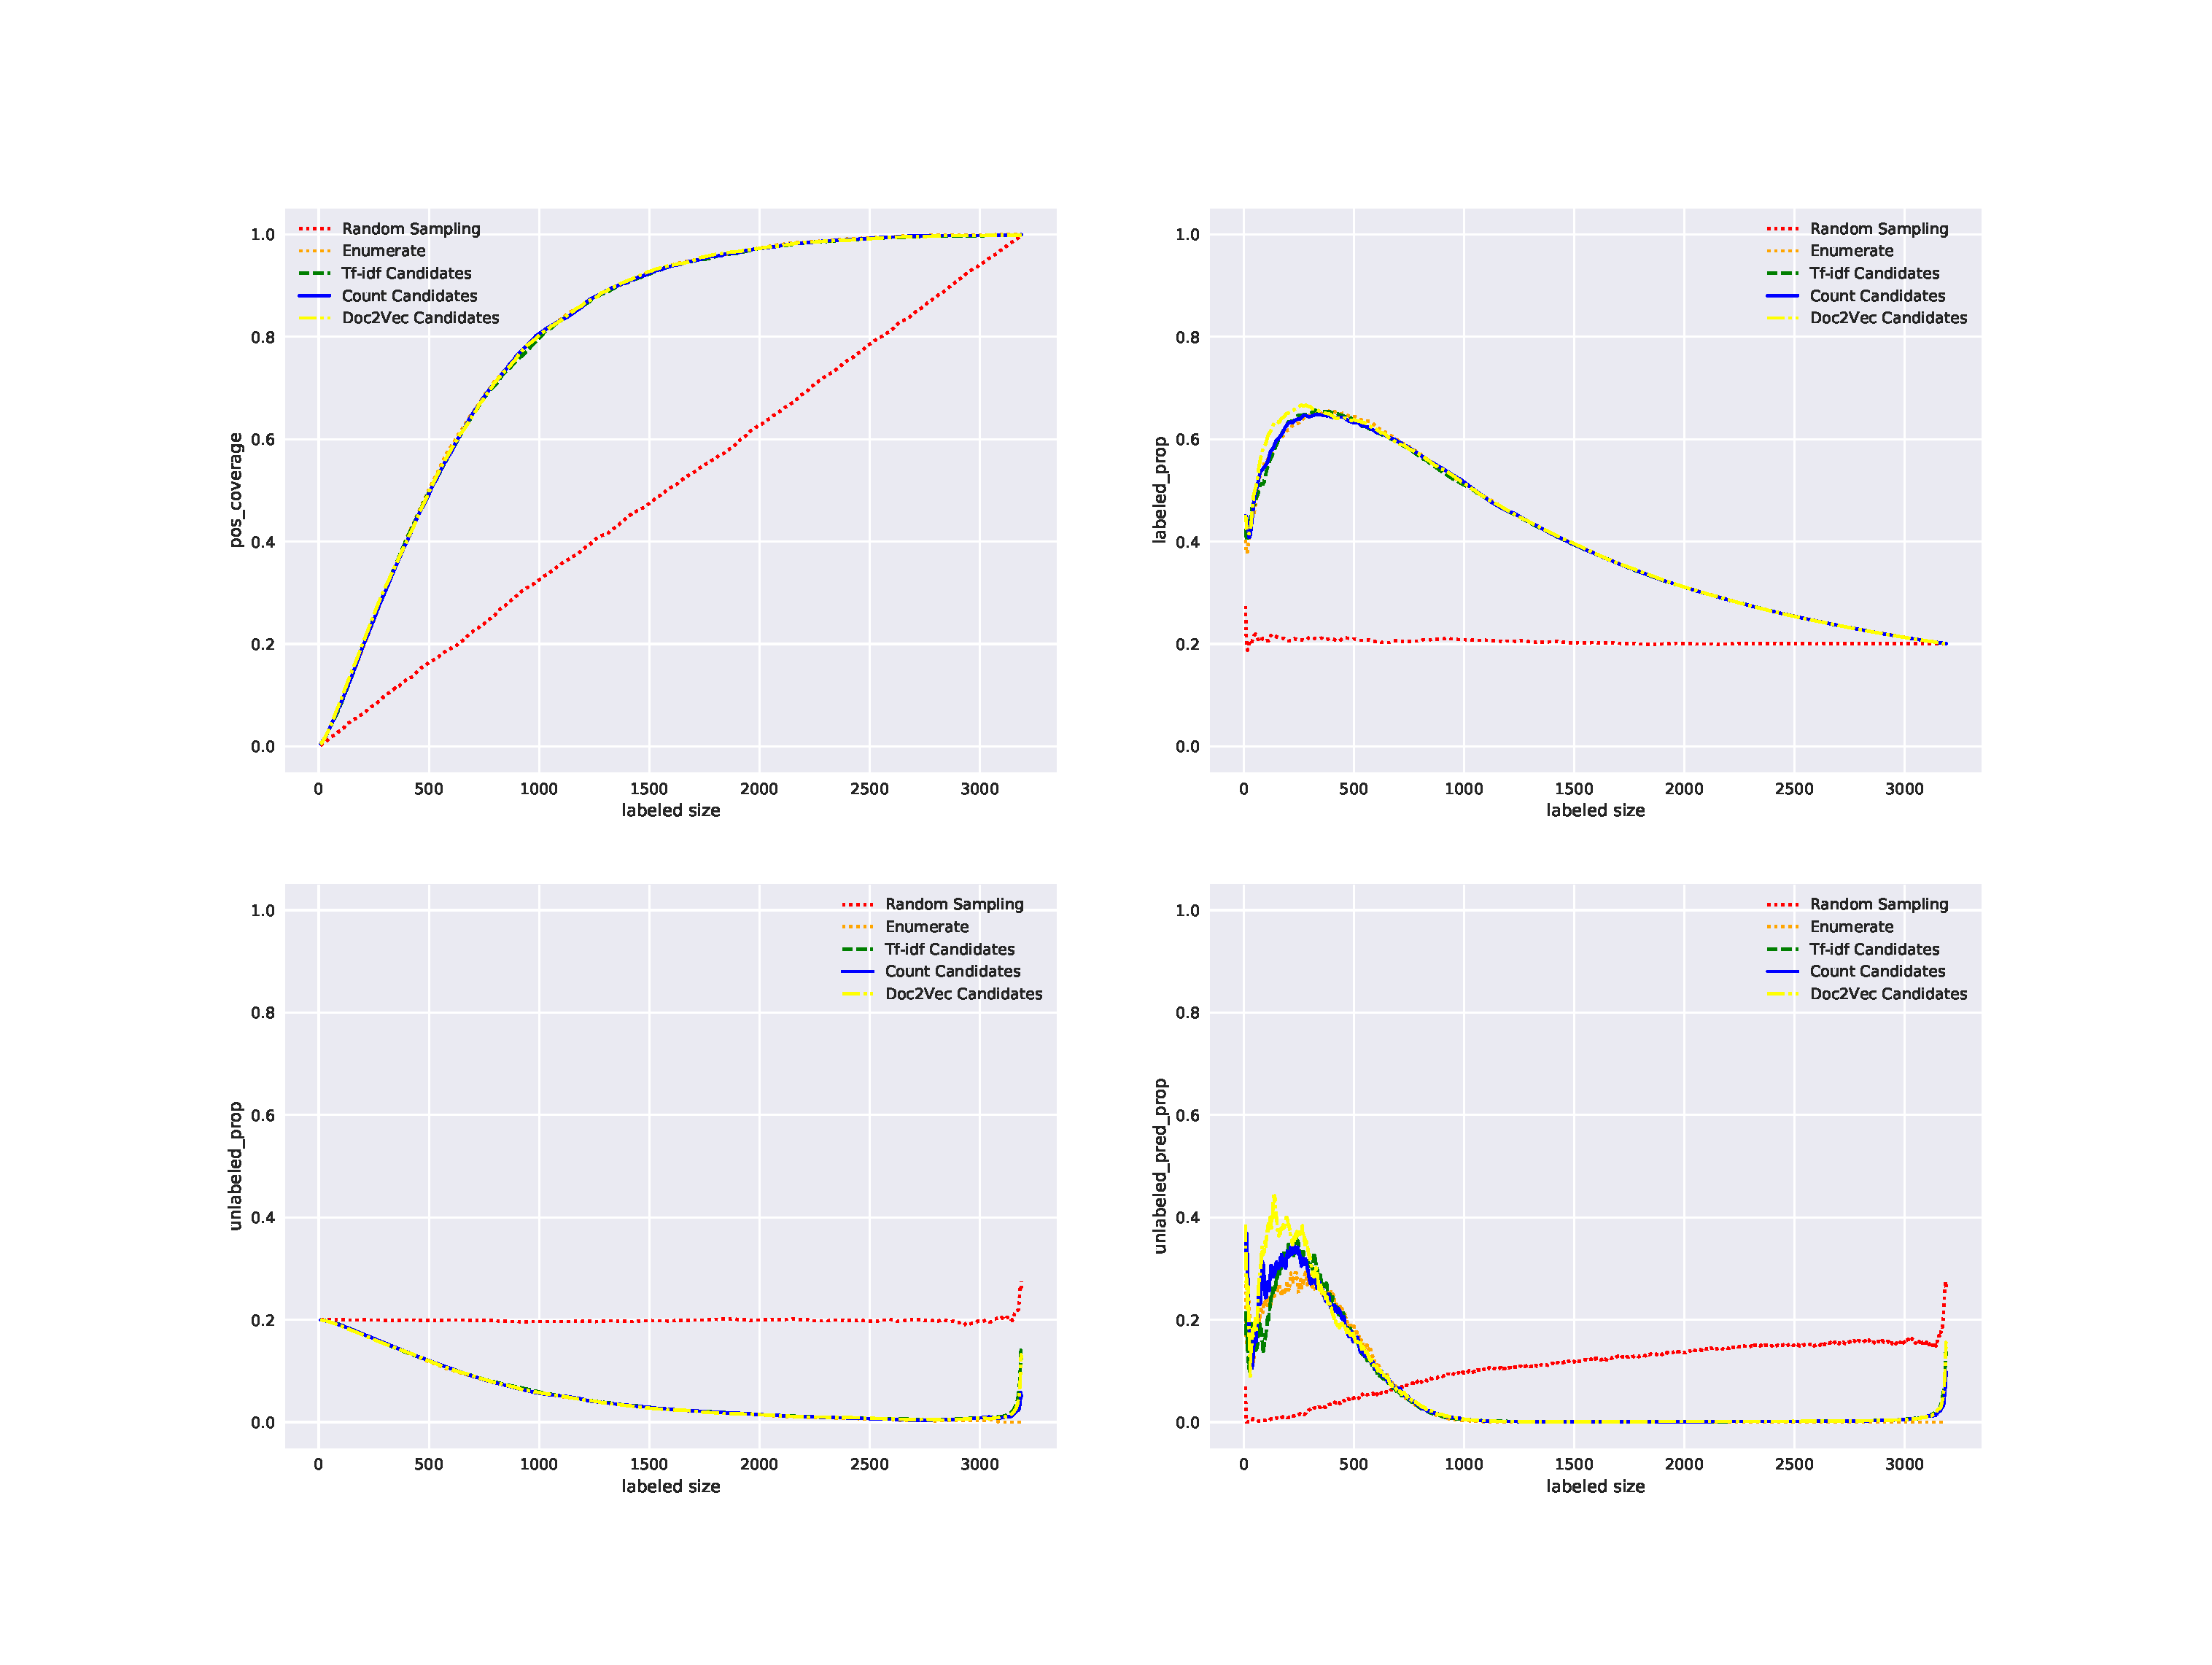
\includegraphics[width=\textwidth]{img/imdb_20/enumerate.eps}
\captionof{figure}{Target Retrieval on Dataset 2}
\label{enumerate2}
\end{figure}

\begin{figure}[!t]
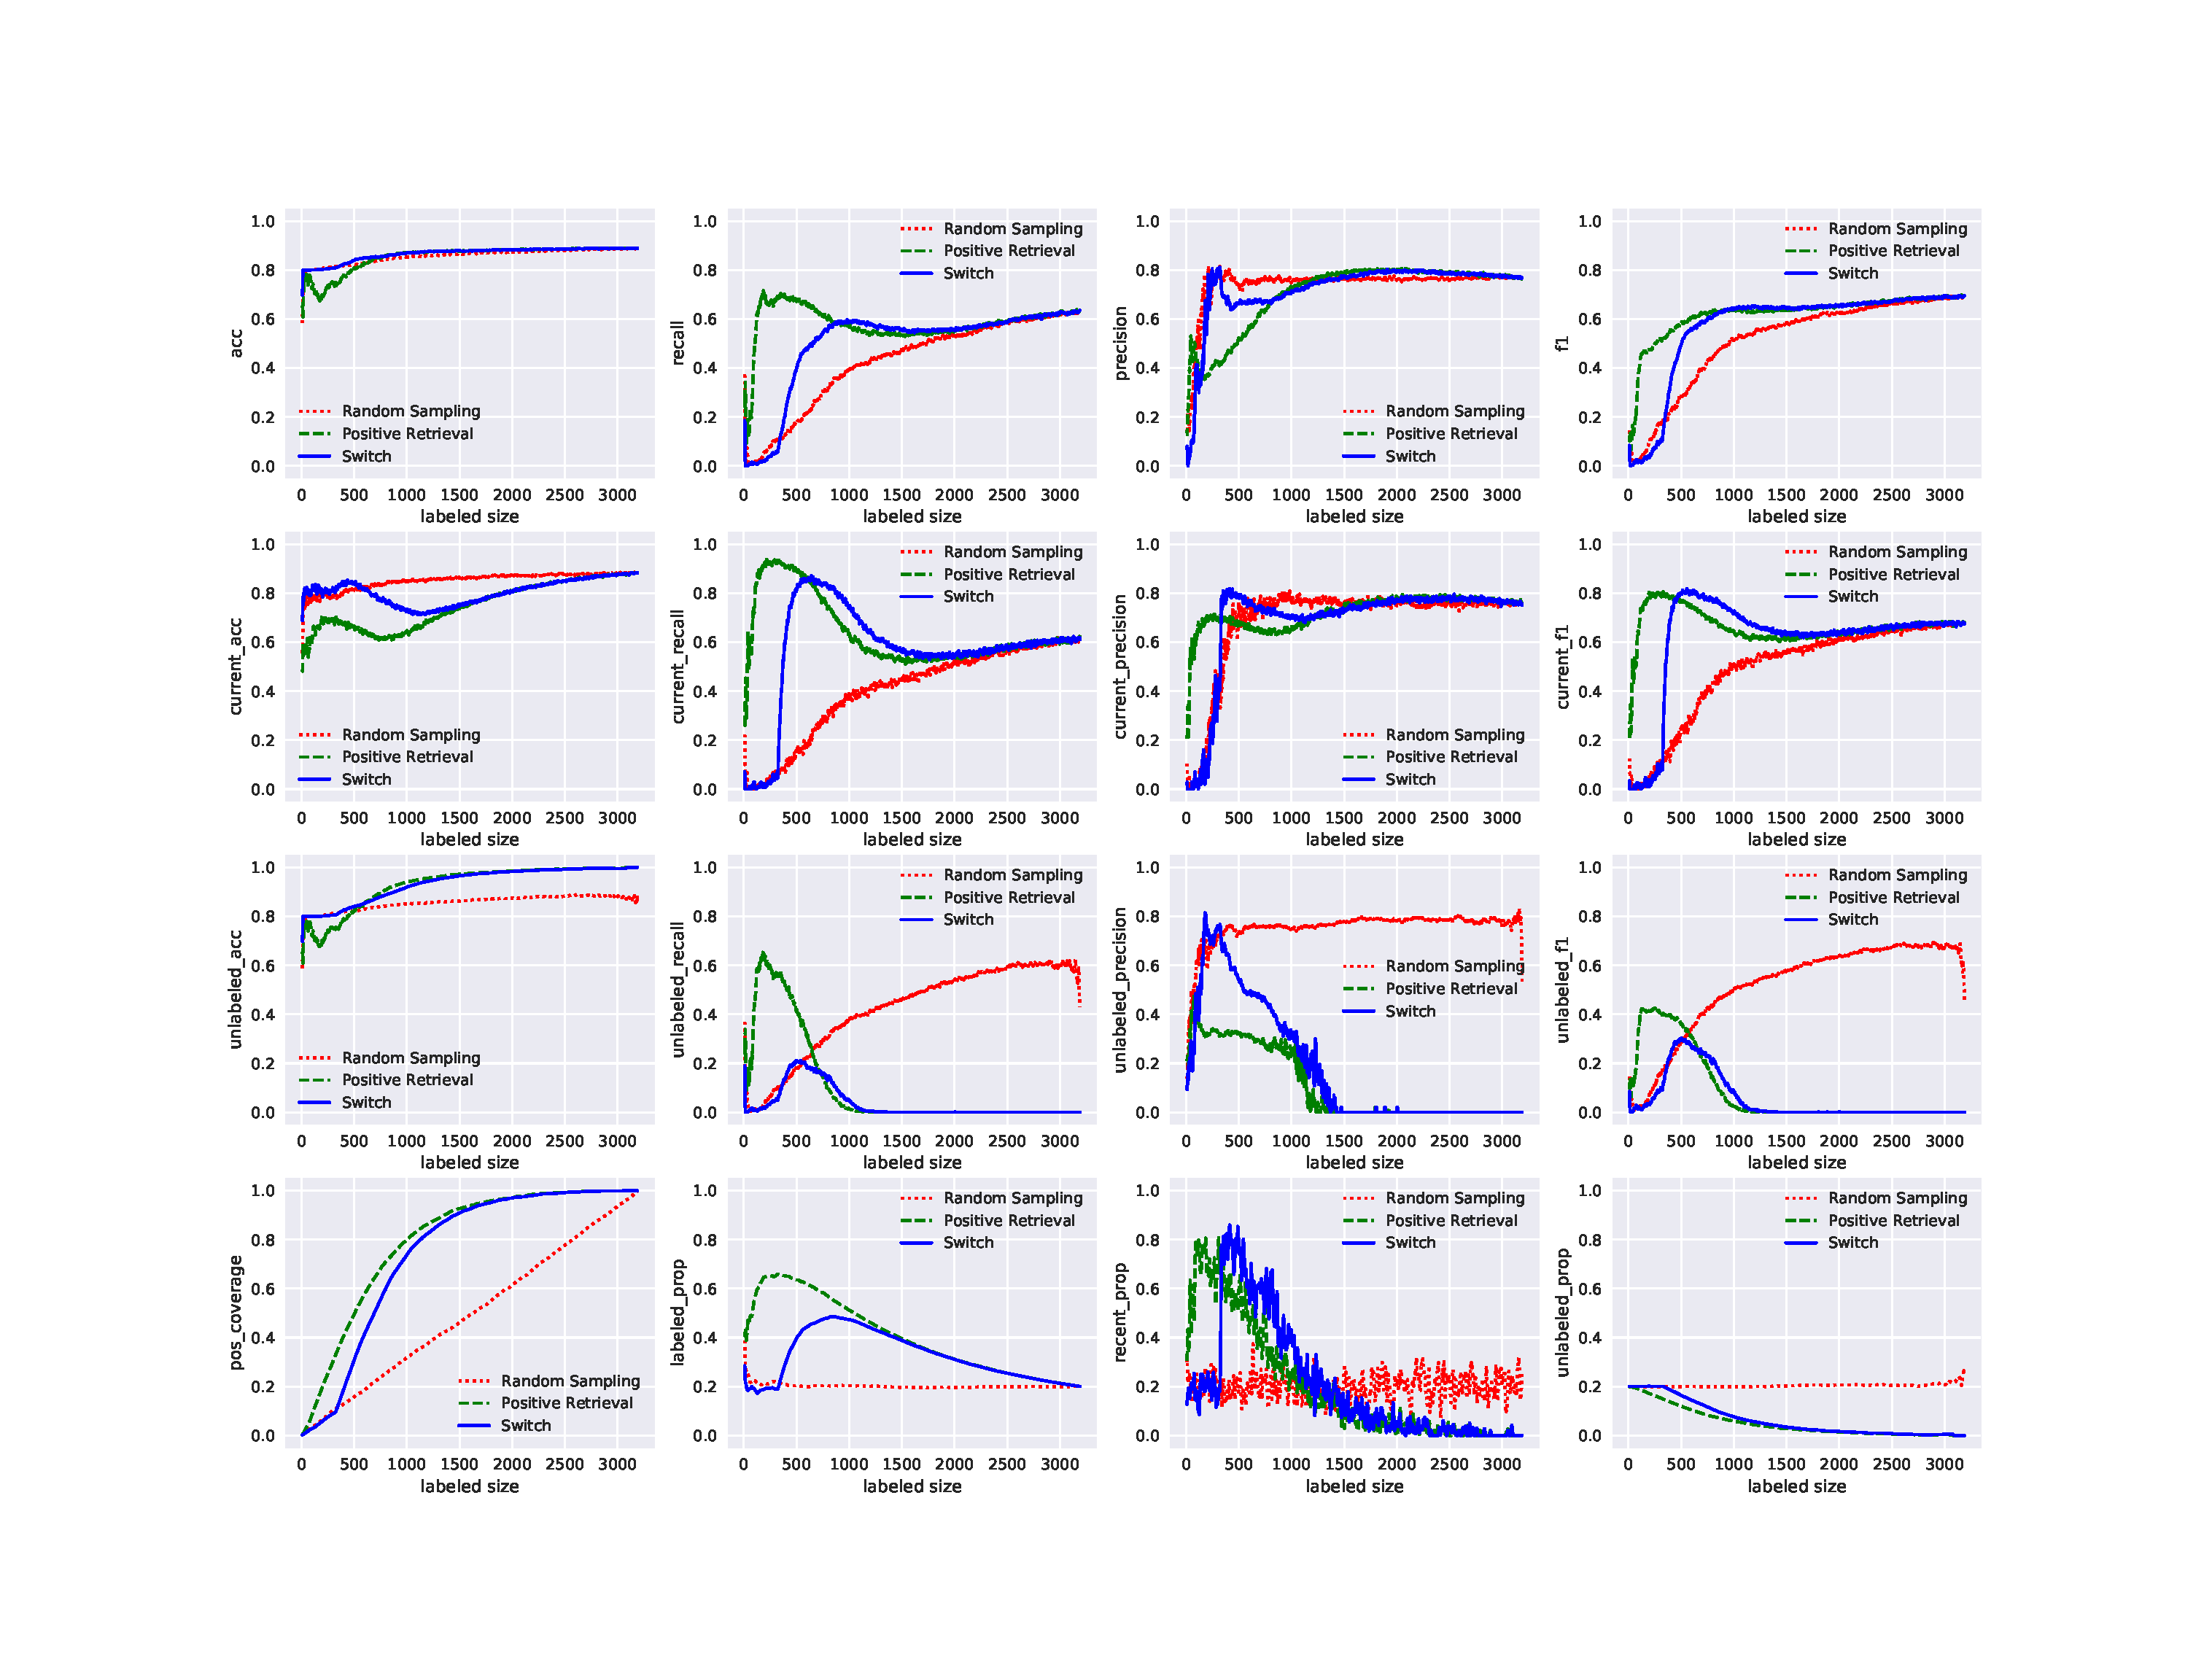
\includegraphics[width=\textwidth]{img/imdb_20/metrics.eps}
\captionof{figure}{Metrics on Dataset 2}
\label{metrics2}
\end{figure}

\begin{figure}[!t]
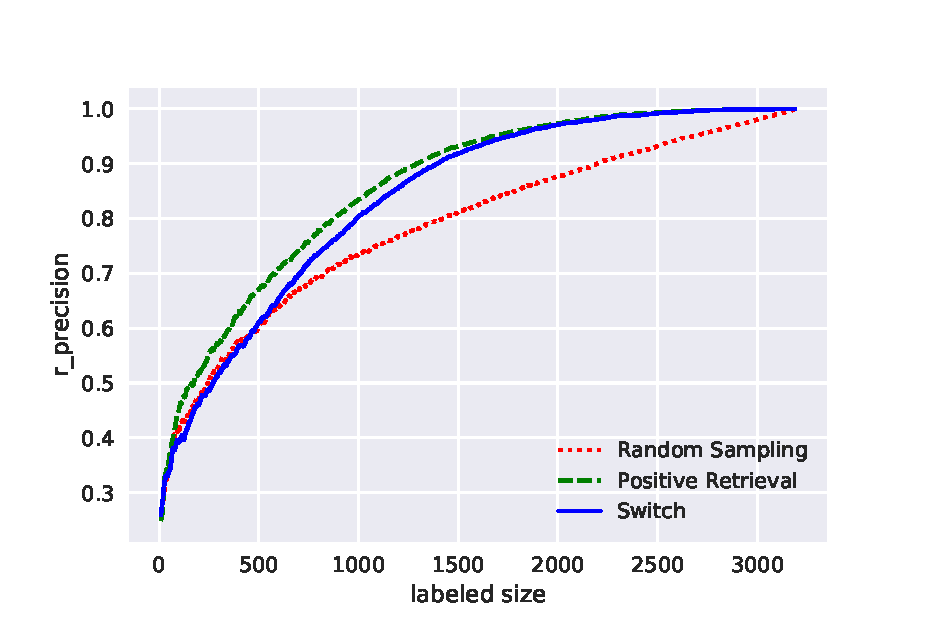
\includegraphics[width=0.6\textwidth]{img/imdb_20/rprecision.eps}
\centering
\captionof{figure}{R-Precision on Dataset 2}
\label{rprecision2}
\end{figure}

\begin{figure}[!t]
\includegraphics[width=\textwidth]{img/imdb_20/heat_map.eps}
\captionof{figure}{Heat Map on Dataset 2}
\label{heatmap2}
\end{figure}

\begin{figure}[!t]
\includegraphics[width=\textwidth]{img/imdb_20/true_heat_map.eps}
\captionof{figure}{Heat Map of True Layer on Dataset 2}
\label{true_heatmap2}
\end{figure}

\begin{figure}[!t]
\includegraphics[width=\textwidth]{img/imdb_20/false_heat_map.eps}
\captionof{figure}{Heat Map of False Layer on Dataset 2}
\label{false_heatmap2}
\end{figure}

\subsubsection{Improving the Performance of Obtained Model}
Since this is an unbalanced dataset, accuracy only will no longer enough to evaluate the performance of the model. In this part, I will focus on f1-score. Figure \ref{performance-base2} and \ref{performance-combine2} show the performance of base methods and combination methods on oracle test set, and I should focus on the AUC of these metrics, which reflects the ``speed'' on a certain level. Firstly, if I compare the two baselines, it is obvious that uncertainty sampling performed much better than random sampling on this dataset. For the base proposed methods, I can find out that methods using tf-idf summation and unique word count did not give better performance than either random sampling or uncertainty sampling. However, Doc2Vec norm method gave an obviously better result than random sampling, but did not exceed uncertainty sampling. For combination methods, methods using tf-idf summation and unique word count did not give better performance than uncertainty sampling baseline either, while Doc2Vec norm method showed a little better performance than uncertainty sampling baseline.

\subsubsection{Finding Data from Target Class Faster}
Figure \ref{enumerate2} shows metrics to measure how fast the model find target data. From positive coverage, I can find out that random sampling baseline also gives a linear result, and learning-to-enumerate baseline gives a much better performance than random sampling, same as on Dataset 1. However, my proposed methods does not give obvious better results than learning-to-enumerate baseline, but if I look at target proportion of labeled data, it is able to say that Doc2Vec Candidates method gives a little better performance.

\subsubsection{Tackling the Performance-Target Dilemma}
From the aspect of giving estimation, I can easily find out in Figure \ref{metrics2} that the pit comes earlier than balanced dataset. Remember the f1-score on oracle test set of Dataset 1, the model with target-retrieval method learned much slower than random sampling, due to the bias towards target data. However, in unbalanced dataset, model with target-retrieval method learned much faster than random sampling baseline. This is because the model tried to fetch target data, which is minority in unlabeled data pool, so that the model was able to learn on a more balanced dataset than random sampling. In this way, target-retrieval method not only fetched target data faster, but contributed to model performance as well. Hence, I can imagine that if the target data is majority in the unlabeled pool, the model will learn on a even more unbalanced dataset, the performance will go worse than random sampling.

Then let us look at heat maps. From Figure \ref{heatmap2}, \ref{true_heatmap2} and \ref{false_heatmap2}, I can find out that it showed obviously different distributions between true layer and false layer in random sampling, but in target-retrieval, heat maps of true layer and false layer almost give same results. A possible reason could be that in target-retrieval method, the learned decision boundary may be different from random sampling. The fortunate thing is that there is no need to focus on the decision boundary, instead, I focus on the target likelihood ranking which is shown in Figure \ref{rprecision2}. I can see that on this unbalanced Dataset 2, random sampling and target-retrieval gave the opposite results to those on balanced Dataset 1. This is easy to understand because a well-learned model should provide a better ranking of target likelihood. I can conclude that the switch method gives a medium performance of R-precision on both balanced and unbalanced datasets.

\chapter{Discussion}

In this chapter, I will summarize the conclusions from the experimental results, and discuss further possibilities.

\section{Conclusion}
In this research, I compared several ways of extracting target data from a fixed unlabeled data pool, not only from the aspect of typical active learning, but also defined a new problem called target-retrieval-learning. I focused on document classification tasks, and I proposed several methods to determine the informative level of a document. Experimental results have shown that base methods did not exceed uncertainty sampling baseline, but method using Doc2Vec norm gave a little but stable better performance than random sampling baseline. Besides, I proposed combination methods with uncertainty sampling and learning-to-enumerate algorithm, and these combination methods have shown little but obvious improvement than baselines on balanced data. But for target-retrieval-learning problem, combination methods showed same level results to baselines. This may be because that target data is already minority in the original distribution, subtle changes may not be obvious comparing to learning-to-enumerate baseline.

When people need to solve the target-retrieval-learning problem on a large dataset, it is often too expensive to have human annotation on all samples. In such cases, people may want to train a supervised machine learning model on the labeled samples, and let the model to predict the class of the remaining unlabeled samples. However, there is a dilemma between improving the performance of model and finding target data fast. The problem is that the priori of the training data will change. As a result, it is difficult to estimate the real performance of the current obtained model. To demonstrate this problem, I built a framework to simulate the annotation process. Meanwhile, I also evaluated several metrics to analyze possible reasons, and tried to estimate the performance and give a target likelihood ranking on unlabeled data, by means of the curves of these metrics. One possible solution is that it is able to observe the ``pit'' in current test set. If the model performs stably after the pit, it is able to switch to the model prediction and do not require human annotation anymore. Also I discussed an approach of switching from random sampling to target retrieval method, which is a trade-off between model performance and target data finding, and helps to give a glance at the original distribution of unlabeled pool. From the aspect of target likelihood ranking, I can conclude that the switch method always give a compromised result on both balanced and unbalanced data.

\section{Further Issues}
In this research, I try to measure the informative level of documents in several ways using text-base properties such as number of bag-of-words features, tf-idf scores and document vector norm. There must be other ways of informative measurement, and I would like to explore more measurement in the future work. Another point is that although the is existing research has shown that norm of Word2Vec vector could be considered as a measurement of word significance, there is not enough evidence about whether other word embeddings (such as GloVe) have similar effect, and whether Doc2Vec vector could represent document significance. I should do more analysis on word embedding and document vector.

I also try to give an estimation about the model on the unlabeled data. However, the estimation is still ambiguous, only providing the information of whether the model is trained acceptably or not, not giving any precise value of evaluation. There may any ways, in which I can make use of statistics to give an approximate expectation and variance of certain metrics on the oracle test set. In actual application, if expectation and variance of f1-score are given, people will be able to make much more reasonable decisions.

\chapter*{Acknowledgements}
\addcontentsline{toc}{chapter}{\numberline{}Acknowledgements}
I would first like to thank my supervisor Professor Tajima of the Department of Social Informatics at Kyoto University. He was offering his precious time every week to check my progress and discuss about the future plans. He was always being patient when I got in trouble with my research or experiments, and gave many important directions about my research. Many thanks!

I would also like to thank Professor Yamakata, associate professor of my laboratory. Although she came to my laboratory from my second year of master course, she was quite eager to help my research, and gave a lot of valuable advice about the background and proposed methods of my research. 

Finally, I must express my very profound gratitude to my advisors, Professor Jatowt and Professor Matsubara, both are associate professor of the Department of Social Informatics. They have been my advisors for these two years. They pointed out several problems in my research, and provided advice of improvement. Thank you.

\createbiblio{references}
\addcontentsline{toc}{chapter}{\numberline{}Bibliography}

\end{document}
